\ifx\allfiles\undefined
\documentclass[12pt, a4paper, oneside, UTF8]{ctexbook}
\def\path{../config}
\usepackage{amsmath}
\usepackage{amsthm}
\usepackage{amssymb}
\usepackage{graphicx}
\usepackage{mathrsfs}
\usepackage{enumitem}
\usepackage{geometry}
\usepackage[colorlinks, linkcolor=black]{hyperref}
\usepackage{stackengine}
\usepackage{yhmath}
\usepackage{extarrows}

\usepackage{multicol}
\usepackage{fancyhdr}
\usepackage[dvipsnames, svgnames]{xcolor}
\usepackage{listings}
\usepackage{subfigure}
\usepackage{tikz}


\definecolor{mygreen}{rgb}{0,0.6,0}
\definecolor{mygray}{rgb}{0.5,0.5,0.5}
\definecolor{mymauve}{rgb}{0.58,0,0.82}

\graphicspath{ {figure/},{../figure/}, {config/}, {../config/} }

\linespread{1.6}

\geometry{
    top=25.4mm, 
    bottom=25.4mm, 
    left=20mm, 
    right=20mm, 
    headheight=2.17cm, 
    headsep=4mm, 
    footskip=12mm
}

\setenumerate[1]{itemsep=5pt,partopsep=0pt,parsep=\parskip,topsep=5pt}
\setitemize[1]{itemsep=5pt,partopsep=0pt,parsep=\parskip,topsep=5pt}
\setdescription{leftmargin=4em,itemsep=5pt,partopsep=0pt,parsep=\parskip,topsep=5pt}

\lstset{
    language=Mathematica,
    basicstyle=\tt,
    breaklines=true,
    keywordstyle=\bfseries\color{NavyBlue}, 
    emphstyle=\bfseries\color{Rhodamine},
    commentstyle=\itshape\color{black!50!white}, 
    stringstyle=\bfseries\color{PineGreen!90!black},
    columns=flexible,
    numbers=left,
    numberstyle=\footnotesize,
    frame=tb,
    breakatwhitespace=false,
} 
% 定理环境
\usepackage{tcolorbox}
\tcbuselibrary{most}
\theoremstyle{definition}


\newtheorem{proposition}{\indent 命题}[section]
\newtheorem{example}{\indent \color{SeaGreen}{例}}[section]
\theoremstyle{plain}
\newtheorem*{rmk}{\indent 注}
\renewenvironment{proof}{\indent\textcolor{SkyBlue}{\textbf{证明.}}\;}{\qed\par}
\newenvironment{solution}{\indent\textcolor{SkyBlue}{\textbf{解.}}\;}{\qed\par}
% #### 将 config.tex 中的定理环境的对应部分替换为如下内容
% 定义单独编号,其他四个共用一个编号计数 这里只列举了五种,其他可类似定义(未定义的使用原来的也可)
\newtcbtheorem[number within=section]{defn}%
{定义}{colback=OliveGreen!10,colframe=Green!70,fonttitle=\bfseries}{def}

\newtcbtheorem[number within=section]{lemma}%
{引理}{colback=Salmon!20,colframe=Salmon!90!Black,fonttitle=\bfseries}{lem}

% 使用另一个计数器 use counter from=lemma
\newtcbtheorem[use counter from=lemma, number within=section]{them}%
{定理}{colback=SeaGreen!10!CornflowerBlue!10,colframe=RoyalPurple!55!Aquamarine!100!,fonttitle=\bfseries}{them}

\newtcbtheorem[use counter from=lemma, number within=section]{criterion}%
{准则}{colback=green!5,colframe=green!35!black,fonttitle=\bfseries}{cri}

\newtcbtheorem[use counter from=lemma, number within=section]{corollary}%
{推论}{colback=Emerald!10,colframe=cyan!40!black,fonttitle=\bfseries}{cor}
% colback=red!5,colframe=red!75!black

% 这个颜色我不喜欢
%\newtcbtheorem[number within=section]{proposition}%
%{命题}{colback=red!5,colframe=red!75!black,fonttitle=\bfseries}{cor}

% .... 命题 例 注 证明 解 使用之前的就可以(全文都是这种框框就很丑了),也可以按照上述定义 ...
\def\d{\mathrm{d}}
\def\R{\mathbb{R}}
\def\C{\mathbb{C}}
\def\a{\bs{a}}
\def\b{\bs{b}}
\def\x{\bs{x}}
\def\y{\bs{y}}
\def\z{\bs{z}}
\def\u{\bs{u}}
\def\A{\bs{A}}
\def\B{\bs{B}}
\def\D{\bs{D}}
\def\G{\bs{G}}
\def\H{\bs{H}}
\def\L{\bs{L}}
\def\Q{\bs{Q}}
\def\X{\bs{X}}
\def\Y{\bs{Y}}
\def\Z{\bs{Z}}
\def\U{\bs{U}}
\def\V{\bs{V}}
\def\P{\bs{P}}
\def\J{\bs{J}}
\def\I{\bs{I}}
\def\E{\bs{E}}
\newcommand{\bs}[1]{\boldsymbol{#1}}
\newcommand{\ora}[1]{\overrightarrow{#1}}
\newcommand{\myspace}[1]{\par\vspace{#1\baselineskip}}
\newcommand{\xrowht}[2][0]{\addstackgap[.5\dimexpr#2\relax]{\vphantom{#1}}}
\newenvironment{ca}[1][1]{\linespread{#1} \selectfont \begin{cases}}{\end{cases}}
\newenvironment{vx}[1][1]{\linespread{#1} \selectfont \begin{vmatrix}}{\end{vmatrix}}
\newcommand{\tabincell}[2]{\begin{tabular}{@{}#1@{}}#2\end{tabular}}
\newcommand{\pll}{\kern 0.56em/\kern -0.8em /\kern 0.56em}
\newcommand{\dive}[1][F]{\mathrm{div}\;\bs{#1}}
\newcommand{\rotn}[1][A]{\mathrm{rot}\;\bs{#1}}
\newcommand{\rank}{\text{rank}}

\def\myIndex{0}
% \input{\path/cover_package_\myIndex.tex}

\def\myTitle{矩阵理论复习笔记}
\def\myAuthor{}
\def\myDateCover{}
\def\myDateForeword{\\\today}
\def\myForeword{前言}
\def\myForewordText{\par
本复习笔记是我个人在学习矩阵理论的过程中整理、总结而成,包含课本的内容、上课PPT涉及到的内容以及不懂地方的补充知识,希望能够对你有所帮助。\par 全书排版是利用\LaTeX 完成的,这也是对我使用\LaTeX 的一次较大工程的练手,希望我能在撰写完之后对于\LaTeX 使用有更深层次的理解。\par 因本人水平有限,故本总结笔记如有不当之处,敬请指出,本人不胜感激!
}
\def\mySubheading{}


\begin{document}

\else
\fi
\chapter{向量与矩阵的范数}
本章将会介绍范数这一概念,主要内容包括介绍向量的范数、矩阵的范数和算子范数,同时在本章的最后会介绍范数的相关应用——借助范数来判断一个矩阵的逆矩阵或求解线性方程组因摄动带来的误差是否处于一个可接受的范围内。

为什么要引入范数?在本章中应时刻牢记范数是一个数而非其他之物,将矩阵、向量类的抽象概念转换成一个“大小”往往能够简化问题。

本章将会涉及到以下内容:
\begin{itemize}[leftmargin=4em]
    \item 向量的范数
    \item 矩阵的范数
    \item 算子范数
    \item 范数的应用
\end{itemize}
\noindent

\textbf{注意}:本章内的内容具有强连续性,需要按照顺序从头开始了解,同时,本章内容会涉及多个定理、性质的证明,需要静下心来仔细复盘证明方法,但本章内容与第一章的联系不大,因此如果觉得第一章理解起来有难度可以先跳过第一章的内容继续学习第二章。
\newpage
\section{向量的范数}
本节我们首先介绍向量的范数,在开始详细介绍向量的范数前我们可以先简单“感受”一下何为范数。
\subsection{范数的直观感受}
在第一章,我们了解过向量的长度:
\[\Vert \bs{x}\Vert=\sqrt{<\bs{x},\bs{x}>}=\bs{x}^H\bs{x}\]

有了向量的长度,向量便在实际空间内有了意义,也给后续定义距离等概念打下了基础。

其实,向量的距离就是向量的2-范数,范数的种类有很多,每一种范数的计算方法都不一样但大同小异,这里利用向量2-范数作说明是因为向量的2-范数便于理解(距离),同时也引出下面的对范数的意义的概括:这便是范数的具体意义——对“距离”概念的延伸,是一种广义的“长度”。

为什么说是广义的“长度”呢?继续阅读就会发现,向量范数并不止向量的2-范数,还有其他类型的向量范数。

\begin{defn}{向量范数的定义}{def:2.1.1}
    设映射$\Vert \bs{\cdot}\Vert: \mathbb{C} ^n\rightarrow \mathbb{R} $满足:
    \begin{enumerate}
        \item 正定条件:$\Vert \bs{x}\Vert\geq0$, 当且仅当$\bs{x=0}$时$|\bs{x}|=0$
        \item 齐次条件:$\Vert \lambda\bs{x}\Vert=|\lambda|\Vert\bs{x}\Vert,\lambda\in\mathbb{C} ,\bs{x}\in\mathbb{C}^n$
        \item 三角不等式:$\Vert\bs{x+y}\Vert\leq+\Vert\bs{y}\Vert,\forall \bs{x,y}\in\mathbb{C}^n$
    \end{enumerate}
    则称映射$\Vert\bs{\cdot}\Vert$为$\mathbb{C}^n$上向量$\bs{x}$的范数,定义了范数的$\mathbb{C}^n$又叫做一个线性赋范空间。
\end{defn}

定义\ref{def:def:2.1.1}给出了能够成为向量范数的条件:是一个映射,并且能够满足三个条件,就可以将这种映射叫做向量的范数,这也是今后判断给出一种映射是否为向量范数的方法。
\subsection{向量范数的性质}{\label{sec:2.1.2}}
定义\ref{def:def:2.1.1}中给出的能够成为向量范数的三个条件也是向量范数的三个性质,除此之外,根据上面的定义,我们还可以得出向量范数的下列性质:
\begin{enumerate}
    \item 零向量的范数是0
    
    这一条性质不难理解,直接使用向量范数的正定条件即可得出。
    \item 当$\bs{x}\neq \bs{0}$时,$\Vert\frac{1}{\Vert\bs{x}\Vert}\bs{x}\Vert=1$
    
    这一条性质通过向量范数的齐次条件可以得出:向量范数是一个数,故$\Vert\frac{1}{\Vert\bs{x}\Vert}\bs{x}\Vert=$

    $\frac{1}{\Vert\bs{x}\Vert}\Vert\bs{x}\Vert=1$
    \item 对任意$\bs{x}\in\mathbb{C}^n$,有$\Vert-\bs{x}\Vert=\Vert\bs{x}\Vert$
    
    同样地,利用齐次性依旧可以得到这一条性质:$\Vert-\bs{x}\Vert=|-1|\cdot\Vert\bs{x}\Vert=\Vert\bs{x}\Vert$

    \item 对任意$\bs{x,y}\in\mathbb{C}^n$,有$|\Vert\bs{x}\Vert-\Vert\bs{y}\Vert|\leq\Vert\bs{x-y}\Vert$
    
    上述不等式的证明过程如下:

    \begin{proof}
        \[
            \Vert\bs{x}\Vert=\Vert\bs{x-y+y}\Vert\leq\Vert\bs{x-y}\Vert+\Vert\bs{y}\Vert(\text{范数的三角不等式})
        \]
    从而
    \[
        \Vert\bs{x-y}\Vert=\Vert\bs{y-x}\Vert\geq \Vert\bs{y}\Vert-\Vert\bs{x}\Vert\text{(依旧是范数的三角不等式)}
    \]
    那么
    \[
        \Vert\bs{x}\Vert-\Vert\bs{y}\Vert\geq -\Vert\bs{x-y}\Vert(\text{不等式左右两边同时乘-1,不等式方向改变})
    \]
    于是就有了
    \[
        |\Vert\bs{x}\Vert-\Vert\bs{y}\Vert|\leq \Vert\bs{x-y}\Vert
    \]
    证毕  
    \end{proof}
\end{enumerate}

\subsection{对向量范数三大性质的理解}
在\ref{sec:2.1.2}节中列出的向量范数的性质,那如何理解向量的范数三大性质呢?

\textbf{对于正定性的理解}:可以从2-范数来看,一般来说,我们认为2-范数表示的是向量的距离,即\[||\bs{x}||_2=\sqrt{x_1^2+x_2^2+\cdots+x_n^2}\](这里$x_1,x_2,\cdots,x_n$代表向量$\boldsymbol{x}$的各个分量),在后面介绍到p-范数的时候也可以从其式子来看出非负性。

\textbf{对于齐次性的理解}:仍以二维空间上的2-范数为例,对于向量$\boldsymbol{x},\lambda\boldsymbol{x}$我们可以将其理解为对该向量进行伸缩变换,当$\lambda$为正时,新的伸缩变换之后的向量与原向量方向相同,当$\lambda$为负时,新的伸缩变换之后的向量与原向量方向相反,由于2-范数描述的为距离,所以$|\lambda|||x||$就代表将向量$\boldsymbol{x}$的距离乘以缩放因子的绝对值(因为范数是个数,所以忽略掉正负带来的影响,因此加绝对值)。

\textbf{对于三角不等式的理解}:依旧以二维空间上的2-范数为例,依据向量相加的平行四边形法则:我们可以画出$\boldsymbol{x}, \boldsymbol{y},\boldsymbol{x+y}$的关系:
\begin{figure}[h]
    \centering
    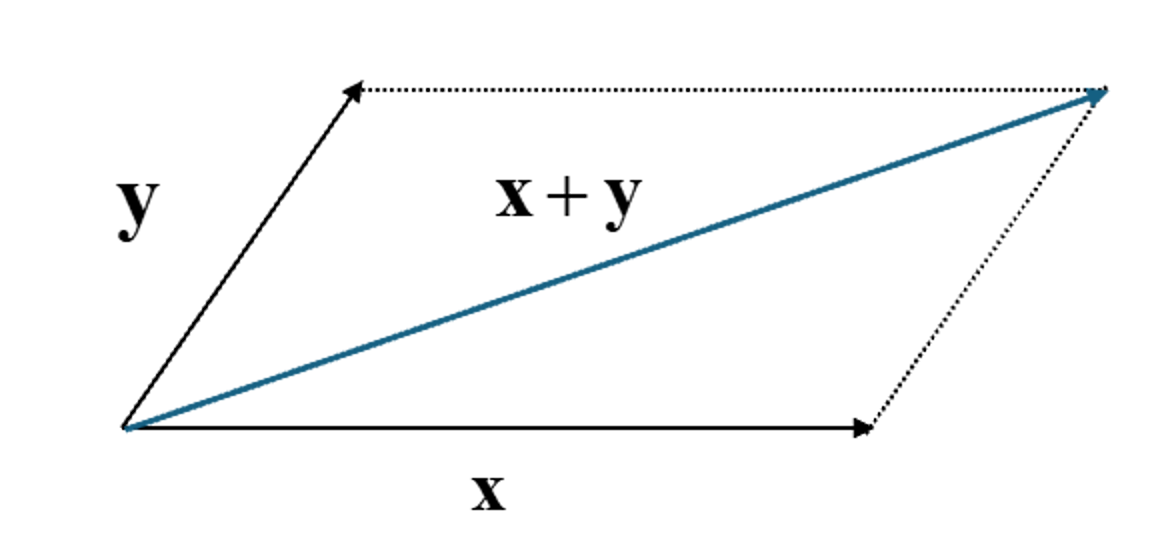
\includegraphics[scale=0.3]{平行四边形法则.png}
\end{figure}

如果我们把向量$\boldsymbol{y}$平移一下,就会得到下面这幅图:
\begin{figure}[h]
    \centering
    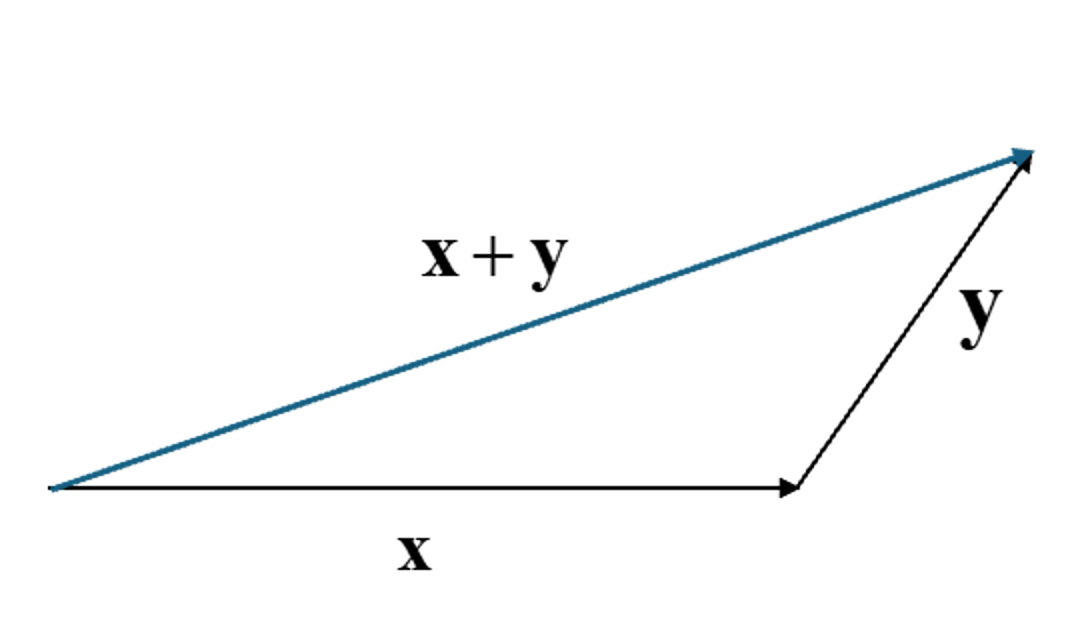
\includegraphics[scale=0.3]{三角形法则.png}
\end{figure}

这就构成了一个三角形,依据三角形两边之和大于第三边的性质,从而可以轻易理解范数性质3——三角不等式的含义。
\subsection{常见的向量范数}{\label{sec2.1.4}}
本节介绍整个向量范数的重点——常见的向量范数
经常使用的向量范数有下面三个:
\[
\begin{aligned}
    \Vert\bs{x}\Vert_1&=\sum\limits_{i=1}^n|x_i|\\
    \Vert\bs{x}\Vert_2&=\left(\sum\limits_{i=1}^n|x_i|^2\right)^{1/2}\\
    \Vert\bs{x}\Vert_{\infty}&=\max\limits_{1\leq i\leq n}|x_i|
\end{aligned}
\]
他们分别为向量1-范数,向量2-范数和向量无穷范数,接下来将会一一给出这三种范数是向量范数的证明。

\subsubsection{向量1-范数的证明与Minkovski不等式}
\noindent
正定性证明:

若向量$\boldsymbol{x}\neq 0$,则表明$\boldsymbol{x}$至少有一个分量$x_k\neq 0$,从而$|x_k|>0$,故$\Vert \boldsymbol{x}\Vert_1>0$

当$\boldsymbol{x=0}$时,显然向量$\boldsymbol{x}$的所有分量必为0,故1-范数一定为0,正定性证毕。

\noindent
齐次性证明:

\[
\begin{aligned}
    \Vert \lambda \boldsymbol{x}\Vert_1&=|\lambda x_1|+|\lambda x_2|+\cdots+|\lambda x_n|\\
    &=|\lambda||x_1|+|\lambda||x_2|+\cdots+|\lambda||x_n|\\
    &=|\lambda|(|x_1|+|x_2|+\cdots+|x_n|)\\
    &=|\lambda|\Vert \boldsymbol{x}\Vert_1
\end{aligned}
\]

齐次性证毕。

\noindent
三角不等式证明:

\[
\begin{aligned}
    \Vert \boldsymbol{x+y}\Vert_1&=\sum_{i=1}^n|x_i+y_i|
\end{aligned}\tag{1}
\]

由$|a+b|\leq |a|+|b|$

式1可以变成\[
\sum_{i=1}^{n}|x_i+y_i|\leq\sum_{i=1}^n|x_i|+\sum_{i=1}^n|y_i|=\Vert \boldsymbol{x}\Vert_1+\Vert\boldsymbol{y}\Vert_1
\]

即
\[
\Vert \boldsymbol{x+y}\Vert_1\leq \Vert \boldsymbol{x}\Vert_1+\Vert\boldsymbol{y}\Vert_1
\]

这个不等式也叫Minkovski不等式。

三角不等式证毕,因此,1-范数是向量范数。

\subsubsection{向量2-范数的证明与Cauchy不等式(柯西不等式)}
在正式介绍向量2-范数之前,需要了解一下关于Cauchy不等式的有关内容。

Cauchy不等式的内容为:
\[|<x,y>|\leq \Vert x\Vert_2\cdot\Vert y\Vert_2\]
即,向量$\boldsymbol{x}$与向量$\boldsymbol{y}$的内积($<\cdot, \cdot>$表示两个向量的内积)的绝对值小于等于两个向量的2-范数。

下面给出在二维欧式空间里Cauchy不等式的证明:

\begin{figure}[h!]
    \centering
    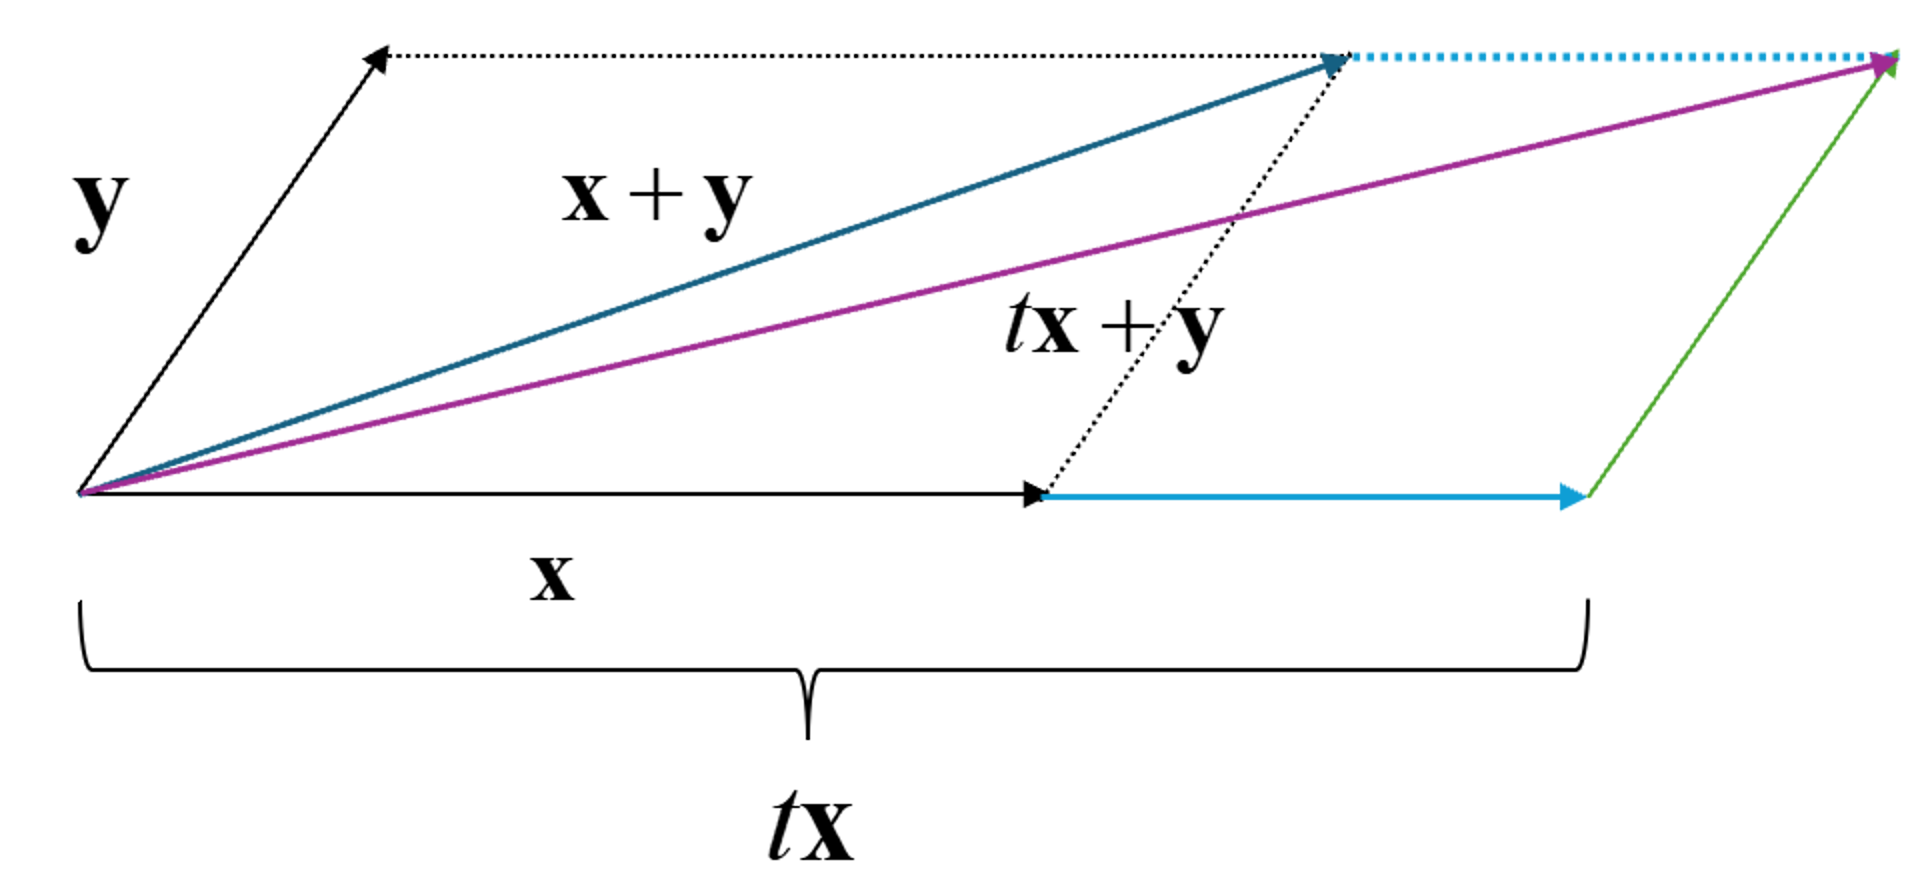
\includegraphics[scale=0.2]{柯西不等式.png}
\end{figure}

如图所示,假设$t>0$,向量$\boldsymbol{x,y,x+y}$和向量$t\boldsymbol{x},y,t\boldsymbol{x+y}$的情况如图,接下来针对向量$\boldsymbol{x}$与向量$\boldsymbol{y}$线性相关与线性无关时分类讨论:

当$\boldsymbol{x}$与向量$\boldsymbol{y}$线性无关时,两个向量的关系可以由上图表示,此时两向量不共线,可由反证法证明得$t\boldsymbol{x+y}\neq\boldsymbol{0}$。

所以
\[\begin{aligned}
|t\boldsymbol{x+y}|^2&=<t\boldsymbol{x+y}, t\boldsymbol{x+y}>\\
&=<\boldsymbol{x,x}>t^2+2<\boldsymbol{x,y}>t+<\boldsymbol{y,y}>
\end{aligned}
\]

这是一个可以看做自变量为$t$的二次函数,令$f(t)=<\boldsymbol{x,x}>t^2+2<\boldsymbol{x,y}>t+<\boldsymbol{y,y}>$。

因为$t\boldsymbol{x}$与$\boldsymbol{y}$线性无关,所以$t\boldsymbol{x+y}\neq\boldsymbol{0}$,故$|t\boldsymbol{x+y}|^2$一定大于0,所以$f(t)>0$。

由于$f(t)$是一个二次函数,二次函数值恒大于零,代表二次函数与$x$轴没有交点,意味着$\triangle=4<\boldsymbol{x,y}>-4<\boldsymbol{x,x}><\boldsymbol{y,y}><0$

即:
\[
<\boldsymbol{x,y}>^2\leq \Vert x\Vert_2^2\Vert y\Vert_2^2
\]

当$\boldsymbol{x}$与向量$\boldsymbol{y}$线性相关时,显而易见,两向量共线,即有关系\[\boldsymbol{y=}t\boldsymbol{x}\]

此时
\[\begin{aligned}
    <\boldsymbol{x},\boldsymbol{y}>^2&=<\boldsymbol{x},\boldsymbol{y}>\cdot<\boldsymbol{x},\boldsymbol{y}>\\
    &=<\boldsymbol{x, kx}>\cdot<\boldsymbol{x, kx}>
    &=k\Vert \boldsymbol{x}\Vert_2^2\cdot k\Vert \boldsymbol{x}\Vert_2^2
    &=k^2\Vert \boldsymbol{x}\Vert_2^2\cdot \Vert \boldsymbol{x}\Vert_2^2\\
    &=\Vert \boldsymbol{y}\Vert_2^2\Vert \boldsymbol{x}\Vert_2^2
\end{aligned}\
\]

故在欧式空间里,Cauchy不等式成立。

需要特别注意的是,上面对于Cauchy不等式的证明是在欧式空间内的,如果放到酉空间中,因为酉空间内$<\boldsymbol{x}, \boldsymbol{y}>$的结果不一定与$<\boldsymbol{y}, \boldsymbol{x}>$的结果相同,故不能进行上面这样的处理,如何证明Cauchy不等式在酉空间内依旧成立呢?请看后续对于Hölder不等式的证明。

接下来开始证明向量2-范数是向量范数:

\noindent
正定性证明:

若向量$\boldsymbol{x}\neq 0$,则表明$\boldsymbol{x}$至少有一个分量$x_k\neq 0$,从而$|x_k|>0$,故$\Vert \boldsymbol{x}\Vert_2>0$

当$\boldsymbol{x=0}$时,显然向量$\boldsymbol{x}$的所有分量必为0,故2-范数一定为0,正定性证毕。

\noindent
齐次性证明:

\[
\begin{aligned}
    \Vert \lambda \boldsymbol{x}\Vert_2&=\sqrt{|\lambda x_1|^2+|\lambda x_2|^2+\cdots+|\lambda x_n|^2}\\
    &=\sqrt{|\lambda|^2|x_1|^2+|\lambda|^2|x_2|^2+\cdots+|\lambda|^2|x_n|^2}\\
    &=|\lambda|\sqrt{|x_1|^2+|x_2|^2+\cdots+|x_n|^2}\\
    &=|\lambda|\Vert \boldsymbol{x}\Vert_2
\end{aligned}
\]

齐次性证毕。

\noindent
三角不等式证明:
\[
\begin{aligned}
    \Vert \boldsymbol{x+y}\Vert_2^2&=<\boldsymbol{x+y,x+y}>\\
    &=(\boldsymbol{x+y})^H(\boldsymbol{x+y})\\
    &=(\boldsymbol{x}^h+\boldsymbol{y}^h)(\boldsymbol{x+y})\\
    &=\boldsymbol{x}^H\boldsymbol{x}+\boldsymbol{x}^H\boldsymbol{y}+\boldsymbol{y}^H\boldsymbol{x}+\boldsymbol{y}^H\boldsymbol{y}\\
    &=|\boldsymbol{x}^H\boldsymbol{x}+\boldsymbol{x}^H\boldsymbol{y}+\boldsymbol{y}^H\boldsymbol{x}+\boldsymbol{y}^H\boldsymbol{y}|\\&(\text{2-范数一般可以理解为长度,长度一定非负,故加绝对值前后大小不变})
\end{aligned}\tag{2}
\]

由$|a+b|\leq |a|+|b|,|ab|=|a|\cdot|b|$

式2可以变为

\[
\begin{aligned}
    |\boldsymbol{x}^H\boldsymbol{x}+\boldsymbol{x}^H\boldsymbol{y}+\boldsymbol{y}^H\boldsymbol{x}+\boldsymbol{y}^H\boldsymbol{y}|&\leq|\boldsymbol{x}^H\boldsymbol{x}|+|\boldsymbol{x}^H\boldsymbol{y}|+|\boldsymbol{y}^H\boldsymbol{x}|+|\boldsymbol{y}^H\boldsymbol{y}|\\
    &=\Vert\boldsymbol{x}\Vert_2^2+2\Vert\boldsymbol{x}\Vert_2\Vert\boldsymbol{y}\Vert_2+\Vert\boldsymbol{y}\Vert_2^2\\
    &=(\Vert\boldsymbol{x}\Vert_2+\Vert\boldsymbol{y}\Vert_2)^2
\end{aligned}
\]

即

\[
\Vert \boldsymbol{x+y}\Vert_2^2\leq(\Vert\boldsymbol{x}\Vert_2+\Vert\boldsymbol{y}\Vert_2)^2
\]
三角不等式证毕,因此,2-范数是向量范数。

\subsubsection{向量无穷范数的证明}
\noindent
正定性证明:

若向量$\boldsymbol{x}\neq 0$,则表明$\boldsymbol{x}$至少有一个分量$x_k\neq 0$,从而$|x_k|>0$,故$\Vert \boldsymbol{x}\Vert_\infty>0$

当$\boldsymbol{x=0}$时,显然向量$\boldsymbol{x}$的所有分量必为0,故无穷范数一定为0,正定性证毕。

\noindent
齐次性证明:

\[
\begin{aligned}
    \Vert \lambda \boldsymbol{x}\Vert_\infty&=\max\limits_{1<i\leq n}|\lambda x_i|\\
    &=|\lambda|\max\limits_{1<i\leq n}|x_i|\\
    &=|\lambda|\Vert \boldsymbol{x}\Vert_\infty
\end{aligned}
\]

齐次性证毕。

\noindent
三角不等式证明:
\[
\begin{aligned}
    \Vert \boldsymbol{x+y}\Vert_\infty=\max\limits_{1<i\leq n}|x_i+y_i|\leq\max\limits_{1<i\leq n}|x_i|+\max\limits_{1<i\leq n}|y_i|=\Vert\boldsymbol{x}\Vert_\infty+\Vert\boldsymbol{y}\Vert_\infty
\end{aligned}
\]

三角不等式证毕,因此,无穷范数是向量范数。

\subsection{向量P-范数}{\label{sec2.1.5}}
在\ref{sec2.1.4}小节中,着重介绍了常见的三种向量范数并给出了其能够成为向量范数的证明,不难发现这三种范数都有一定的相似的结构,能否有一种公式能够总括这些常见的范数呢?

实际上,\ref{sec2.1.4}介绍的三种常见范数都是本小节要介绍的P-范数的特殊情况,向量P-范数又叫做Hölder范数,其形式如下
\begin{defn}{向量P-范数的定义}{def:2.1.2}
    \[\Vert\bs{x}\Vert_p=\left(\sum\limits_{i=1}^n|x_i|^p\right)^{\frac{1}{p}},1\leq p<\infty\]
\end{defn}

通过上面的定义,不难发现,当$p=1$的时候,其为向量1-范数,当$p=2$的时候,其为向量2-范数,当$p\to\infty$的时候,其为向量无穷范数。

那如何证明向量$P$范数依旧是向量范数呢?接下来给出向量$P$范数是向量范数的证明,但在此之前,还需要介绍一些背景知识。

\subsubsection{Young不等式(杨氏不等式)}
接下来介绍Young不等式,Young不等式的内容如下:
若$u$和$v$是非负实数,$p,q$都是正实数,且满足条件$p>1$和$\frac{1}{p}+\frac{1}{q}=1$,则恒有不等式\[uv\leq\frac{1}{p}u^p+\frac{1}{q}v^q\]

下面给出Young不等式的证明:

如下图
\begin{figure}[h]
    \centering
    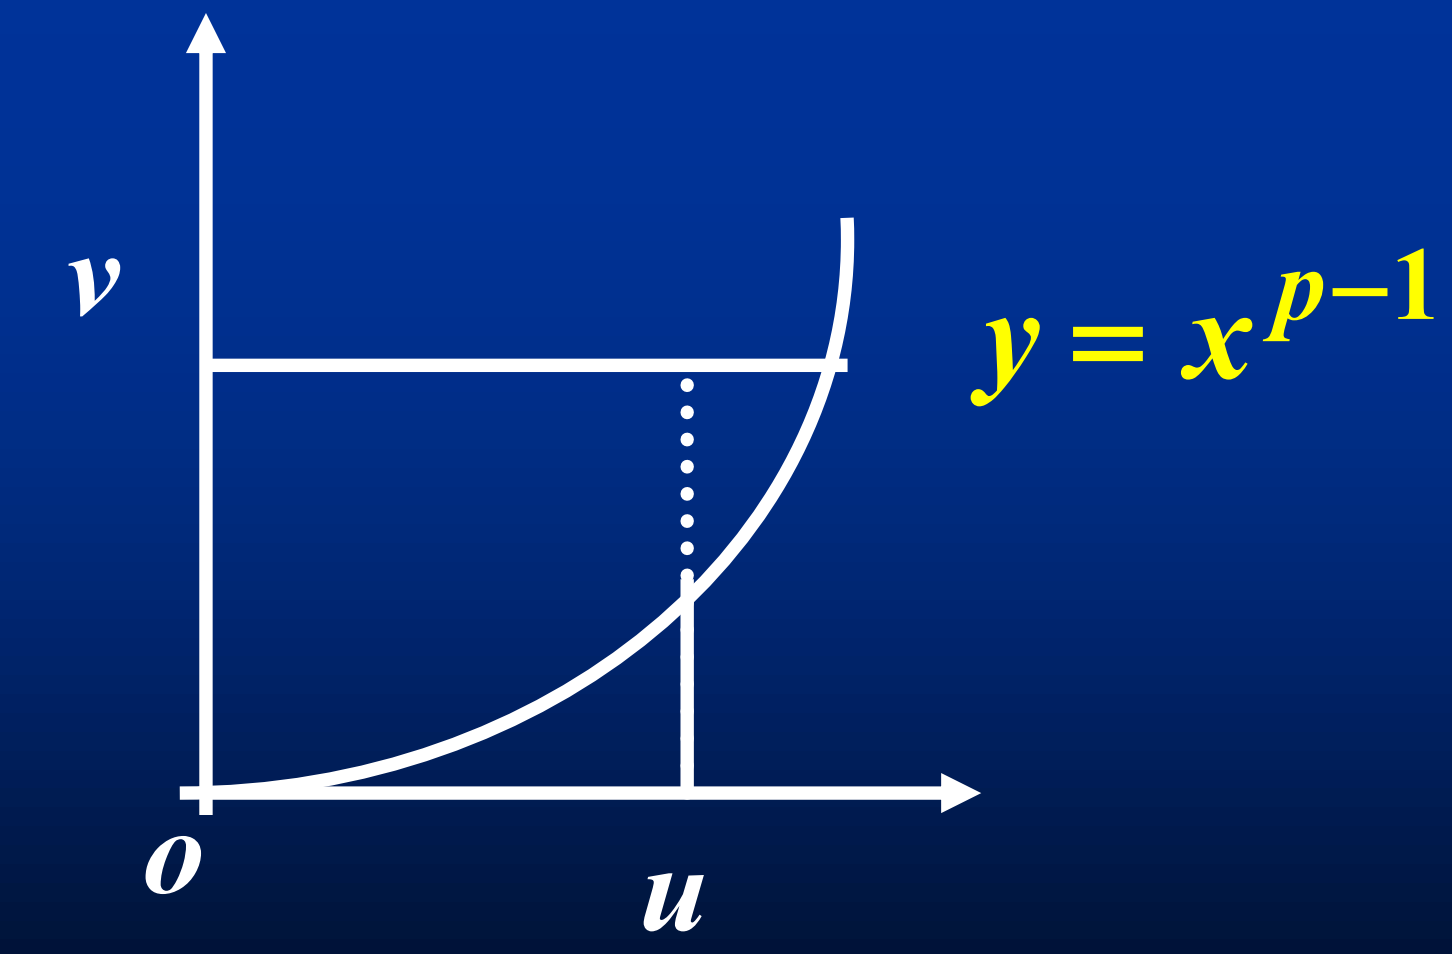
\includegraphics[width=0.25\linewidth]{Young不等式.png}
    \label{fig:enter-label}
\end{figure}

我们可以根据该图得出如下三部分:

\begin{itemize}[leftmargin=4em]
    \item $uv$: 矩形的面积
    \item $\int_0^u x^{p-1}\mathrm{d}x$: 以$(u, u^{p-1})$与$x$轴包裹的小曲面三角形的面积
    \item $\int_0^{v} y^{\frac{1}{p-1}}\mathrm{d}y$: 以$(v^{\frac{1}{p-1}}, v)$与$y$轴包裹的小曲面三角形的面积
\end{itemize}

看图,当$u$与$v$并不相交于函数同一点,即$v\neq u^{p-1}$的时候,很明显能知道矩形的面积是小于两部分曲面三角形的面积的和的,而当$v= u^{p-1}$时,矩形的面积恰好等于两部分曲面三角形的面积的和。

有了上面的认识,接下来将通过严格的数学推导理性的证明Young不等式:

首先,注意到\[\frac{1}{q}+\frac{1}{p}=1\]

对其进行变形,有\[pq=p+q\]

同时,
\[
\begin{aligned}
    \int_0^u x^{p-1}\mathrm{d}x&=\frac{1}{p}x^p|_{x=0}^{x=u}\\
    &=\frac{1}{p}u^p
\end{aligned}
\]

下面处理$\int_0^{v} y^{\frac{1}{p-1}}\mathrm{d}y$:

由Young不等式的前提,得到了$pq=p+q$,从而有\[p=(p-1)q\]

同时有\[\frac{q}{p}=\frac{1}{p-1}\]

所以

\[
\begin{aligned}
    \int_{0}^v y^{\frac{1}{p-1}}\mathrm{d}y&=\int_0^v y^{\frac{q}{p}}\mathrm{d}y\\
    &=\frac{1}{\frac{q}{p}+1}y^{\frac{q}{p}+1}|_{y=0}^{y=v}
    &=\frac{1}{\frac{p+q}{p}}v^{\frac{p+q}{p}}
    &=\frac{1}{\frac{pq}{p}}v^{\frac{pq}{p}}
    &=\frac{1}{q}v^q
\end{aligned}
\]

故\[
uv\leq\frac{1}{p}u^p+\frac{1}{q}v^q 
\]
证毕。
\subsubsection{Hölder不等式}
在\ref{sec2.1.4}节介绍Cauchy不等式的最后提到,用原本的在欧式空间中证明Cauchy不等式在酉空间中依旧成立是不适用的,那应该如何证明在酉空间中,Cauchy不等式依旧成立呢?这就是本节要讨论的Hölder不等式,其内容如下:

若$p,q>1$,且$\frac{1}{p}+\frac{1}{q}=1$,则对$\boldsymbol{C}^n$中任意向量$\boldsymbol{x}=(x_1,x_2,\cdots,x_n)^T, \boldsymbol{y}=(y_1,y_2,\cdots,y_n)^T$都有
\[
\sum\limits_{i=1}^n|x_i||y_i|\leq(\sum\limits_{i=1}^n|x_i|^p)^{1/p}(\sum\limits_{i=1}^n|y_i|^q)^{1/q}
\]

这里看等号右边的这两个乘积项,不难发现这与范数的定义很相似,就是$\Vert \boldsymbol{x}\Vert_p$与$\Vert \boldsymbol{y}\Vert_q$

下面给出Hölder不等式的证明:

令\[u=\frac{|x_i|}{\Vert \boldsymbol{x}\Vert_p},v=\frac{|y_i|}{\Vert \boldsymbol{y}\Vert_q} \]

由Young不等式,可以得到
\[
\begin{aligned}
    uv=\frac{|x_i||y_i|}{\Vert \boldsymbol{x}\Vert_p \Vert \boldsymbol{y}\Vert_q}\leq
    \frac{1}{p}\frac{|x_i|^p}{\Vert \boldsymbol{x}\Vert_p^p}+\frac{1}{q}\frac{|y_i|^q}{\Vert \boldsymbol{y}\Vert_q^q}\ \ \ \ (i=1,2,\cdots,n)
\end{aligned}
\]

等式左右两侧分别进行累加,从$1$加至$n$,从而有
\[
\sum\limits_{i=1}^n\frac{|x_i||y_i|}{\Vert \boldsymbol{x}\Vert_p \Vert \boldsymbol{y}\Vert_q}\leq\frac{1}{p\Vert \boldsymbol{x}\Vert_p^p}\sum\limits_{i=1}^n|x_i|^p+\frac{1}{q\Vert \boldsymbol{y}\Vert_q^q}\sum\limits_{i=1}^n|y_i|^q\tag{1}
\]

由$p$-范数的式子\[
\Vert \boldsymbol{x}\Vert_p=\left(\sum_{i=1}^n|x_i|^p\right)^{1/p}
\]

可以得出\[
\Vert \boldsymbol{x}\Vert_p^p=\sum_{i=1}^n|x_i|^p
\]

从而有
\[\frac{\sum\limits_{i=1}^n|x_i|^p}{\Vert \boldsymbol{x}\Vert_p^p}=1\tag{2}\]

故,不等式1的右侧不等号
\[
\begin{aligned}
\frac{1}{p\Vert \boldsymbol{x}\Vert_p^p}\sum\limits_{i=1}^n|x_i|^p+\frac{1}{q\Vert \boldsymbol{y}\Vert_q^q}\sum\limits_{i=1}^n|y_i|^q=\frac{1}{p}\sum\limits_{i=1}^n\frac{|x_i|^p}{\Vert \boldsymbol{x}\Vert_p^p}
+\frac{1}{q}\sum\limits_{i=1}^n\frac{|y_i|^q}{\Vert \boldsymbol{y}\Vert_q^q}
\end{aligned}\tag{3}
\]

由式2的结果,式3的结果最后为
\[
\frac{1}{p}+\frac{1}{q}=1(\text{根据Young不等式的前提})
\]

故式1化简为
\[
\sum\limits_{i=1}^n\frac{|x_i||y_i|}{\Vert \boldsymbol{x}\Vert_p \Vert \boldsymbol{y}\Vert_q}\leq 1
\]

等式左右两侧同时乘$\Vert \boldsymbol{x}\Vert_p \Vert \boldsymbol{y}\Vert_q$,有

\[
\sum\limits_{i=1}^n|x_i|\cdot|y_i|\leq \Vert \boldsymbol{x}\Vert_p \Vert \boldsymbol{y}\Vert_q
\]

即
\[
\sum\limits_{i=1}^n|x_i||y_i|\leq(\sum\limits_{i=1}^n|x_i|^p)^{1/p}(\sum\limits_{i=1}^n|y_i|^q)^{1/q}
\]
证毕。

上面的是Hölder不等式的全部证明过程,那Hölder不等式与Cauchy不等式的关系是什么呢?

仔细观察Hölder不等式的右侧,可以发现,当$p=q=2$时,这就是Cauchy不等式的右侧,那左侧的$|<\boldsymbol{x,y}>|$要怎么得出来呢?

根据内积的定义,有\[
<\boldsymbol{x,y}>=\boldsymbol{x}^H\boldsymbol{y}=\bar{x}_1y_1+\bar{x}_2y_2+\cdots+\bar{x}_ny_n
\]

故等式两侧都加绝对值,有\[
|<\boldsymbol{x,y}>|=|\boldsymbol{x}^H\boldsymbol{y}|=|\bar{x}_1y_1+\bar{x}_2y_2+\cdots+\bar{x}_ny_n|\tag{4}
\]

根据绝对值三角不等式\[
|a+b|\leq|a|+|b|
\]

式4的结果为\[
|<\boldsymbol{x,y}>|\leq |\bar{x}_1y_1|+|\bar{x}_2y_2|+\cdots+|\bar{x}_ny_n|\tag{5}
\]

又根据性质\[|ab|=|a|\cdot|b|\]

式5的结果为\[
|<\boldsymbol{x,y}>|\leq |\bar{x}_1y_1|+|\bar{x}_2y_2|+\cdots+|\bar{x}_ny_n|=|x_1||y_1|+|x_2||y_2|+\cdots+|x_n||y_n|=\sum\limits_{i=1}^n|x_i||y_i|\tag{5}
\]

所以我们就得出了如下的不等关系:
\[
|<\boldsymbol{x,y}>|\leq\sum\limits_{i=1}^n|x_i||y_i|\leq(\sum\limits_{i=1}^n|x_i|^p)^{1/p}(\sum\limits_{i=1}^n|y_i|^q)^{1/q}
\]

这样,Cauchy不等式在酉空间下依旧成立,证毕。
\subsubsection{P-范数是向量范数的证明}
有了前面这些定理,接下来开始证明P-范数是向量范数:

\noindent
正定性证明:

若向量$\boldsymbol{x}\neq 0$,则表明$\boldsymbol{x}$至少有一个分量$x_k\neq 0$,从而$|x_k|>0$,故$\Vert \boldsymbol{x}\Vert_p>0$

当$\boldsymbol{x=0}$时,显然向量$\boldsymbol{x}$的所有分量必为0,故$p$-范数一定为0,正定性证毕。

\noindent
齐次性证明:

\[
\begin{aligned}
    \Vert \lambda \boldsymbol{x}\Vert_p&=\sqrt[p]{|\lambda x_1|^p+|\lambda x_2|^p+\cdots+|\lambda x_n|^p}\\
    &=\sqrt[p]{|\lambda|^p|x_1|^p+|\lambda|^p|x_2|^p+\cdots+|\lambda|^p|x_n|^p}\\
    &=|\lambda|\sqrt[p]{|x_1|^p+|x_2|^p+\cdots+|x_n|^p}\\
    &=|\lambda|\Vert \boldsymbol{x}\Vert_p
\end{aligned}
\]

齐次性证毕。

\noindent
三角不等式证明:

当$p=1$的时候,很明显,这是1-范数,1-范数的三角不等式证明过程请参见\ref{sec2.1.4}节。

当$p>1$时

\[
\begin{aligned}
    \sum\limits_{i=1}^n(|x_i|+|y_i|)^p&=\sum\limits_{i=1}^n(|x_i|+|y_i|)\cdot(|x_i|+|y_i|)^{p-1}\\
    &=\sum\limits_{i=1}^n|x_i|(|x_i|+|y_i|)^{p-1}+\sum\limits_{i=1}^n|y_i|(|x_i|+|y_i|)^{p-1}
\end{aligned}\tag{8}
\]

由Hölder不等式,式8可以变为
\[
\begin{aligned}
    \sum\limits_{i=1}^n|x_i|(|x_i|+|y_i|)^{p-1}+\sum\limits_{i=1}^n|y_i|(|x_i|+|y_i|)^{p-1}&\leq
    \sum\limits_{i=1}^n\left[(|x_i|+|y_i|)^{(p-1)q}\right]^{\frac{1}{q}}\left(\sum\limits_{i=1}^n|x_i|^p\right)^{\frac{1}{p}}\\&+\sum\limits_{i=1}^n\left[(|x_i|+|y_i|)^{(p-1)q}\right]^{\frac{1}{q}}\left(\sum\limits_{i=1}^n|y_i|^p\right)^{\frac{1}{p}}
\end{aligned}
\]

注意到不等式右侧都有项$\sum\limits_{i=1}^n\left[(|x_i|+|y_i|)^{(p-1)q}\right]^{\frac{1}{q}}$,提取公因式,有

\[
\begin{aligned}
    \left(\left(\sum\limits_{i=1}^n|x_i|^p\right)^{\frac{1}{p}}+\left(\sum\limits_{i=1}^n|y_i|^p\right)^{\frac{1}{p}}\right)\left[\sum\limits_{i=1}^n(|x_i|+|y_i|)^{(p-1)q}\right]^{\frac{1}{q}}
\end{aligned}
\]

所以经过整理,我们得到了下面这个式子:

\[
\sum\limits_{i=1}^n\left(|x_i|+|y_i|\right)^p\leq\left(\left(\sum\limits_{i=1}^n|x_i|^p\right)^{\frac{1}{p}}+\left(\sum\limits_{i=1}^n|y_i|^p\right)^{\frac{1}{p}}\right)\left[\sum\limits_{i=1}^n(|x_i|+|y_i|)^{(p-1)q}\right]^{\frac{1}{q}}\tag{9}
\]

由Young不等式的前提条件(如果忘记了请看1.4节)$p=(p-1)q$,式9可以变为
\[
\sum\limits_{i=1}^n\left(|x_i|+|y_i|\right)^p\leq\left(\left(\sum\limits_{i=1}^n|x_i|^p\right)^{\frac{1}{p}}+\left(\sum\limits_{i=1}^n|y_i|^p\right)^{\frac{1}{p}}\right)\left[\sum\limits_{i=1}^n(|x_i|+|y_i|)^{p}\right]^{\frac{1}{q}}\tag{10}
\]

注意到不等号左右两侧都有项$\sum\limits_{i=1}^n\left(|x_i|+|y_i|\right)^p$,故提公因式,有
\[
\left[\sum\limits_{i=1}^n\left(|x_i|+|y_i|\right)^p\right]^{1-\frac{1}{q}}\leq\left(\left(\sum\limits_{i=1}^n|x_i|^p\right)^{\frac{1}{p}}+\left(\sum\limits_{i=1}^n|y_i|^p\right)^{\frac{1}{p}}\right)\tag{11}
\]

又由Young不等式的前提条件:$\frac{1}{p}+\frac{1}{q}=1$,故式11可以化简为:

\[
\left[\sum\limits_{i=1}^n\left(|x_i|+|y_i|\right)^p\right]^{\frac{1}{p}}\leq\left(\left(\sum\limits_{i=1}^n|x_i|^p\right)^{\frac{1}{p}}+\left(\sum\limits_{i=1}^n|y_i|^p\right)^{\frac{1}{p}}\right)\tag{12}
\]

接下来,只需要证明
\[
\Vert\boldsymbol{x+y}\Vert_p\leq\left[\sum\limits_{i=1}^n\left(|x_i|+|y_i|\right)^p\right]^{\frac{1}{p}}
\]

即可

由$p$-范数的定义和绝对值三角不等式,有
\[
\Vert\boldsymbol{x+y}\Vert_p=\left(\sum\limits_{i=1}^n
(|x_i+y_i|)^p\right)^{\frac{1}{p}}\leq\left(\sum\limits_{i=1}^n
(|x_i|+|y_i|)^p\right)^{\frac{1}{p}}\leq\Vert\boldsymbol{x}\Vert_p+\Vert\boldsymbol{y}\Vert_p
\]

故三角不等式成立,故$p$范数是向量范数,证毕。

证明$p$-范数的三角不等式比较复杂,主要涉及下面五步:
\begin{enumerate}[leftmargin=4em]
    \item 将起点$\sum\limits_{i=1}^n(|x_i|+|y_i|)^p$变换为$1$与$p-1$两个幂相乘的形式,并应用分配律展开。
    \item 在第一步的基础上,应用Hölder不等式进行放大。
    \item 提公因式$\sum\limits_{i=1}^n\left[(|x_i|+|y_i|)^{(p-1)q}\right]^{\frac{1}{q}}$,并应用Young不等式的前提条件进行化简
    \item 不等式左右两侧同时除以$\sum\limits_{i=1}^n\left(|x_i|+|y_i|\right)^p$,并继续应用Young不等式的前提条件进行化简。
    \item 应用$|x_i+y_i|\leq |x_i|+|y_i|$,得到最后的结论。
\end{enumerate}

由此,通过P-范数的定义,我们知道了一个范数有无数种种类描述,并非只有向量1-范数、向量2-范数或向量无穷范数,同时经过\ref{sec2.1.4}和\ref{sec2.1.5}两个小节的介绍,对于向量的范数有了更直观的感受——范数的确是一种广义的“距离”。


\subsection{向量范数的应用}
在本节的最后一小节,介绍一下向量范数的三大应用——利用高维空间的范数定义低维空间的向量范数、向量范数的等价和利用向量范数研究向量序列的收敛性
\subsubsection{利用高维空间的向量范数定义低维空间的向量范数}
\begin{them}{}{them:2.1.1}
    设$\Vert\bs{\cdot}\Vert$是$\mathbb{C}^n$上的范数,$A\in\mathbb{C}_{n}^{m\times n}$(表示$A$矩阵的列数等于矩阵的秩,即$A$矩阵列满秩),则$\Vert A\bs{\cdot}\Vert$是$\mathbb{C}^n$上的范数。
\end{them}
定理$\ref{them:them:2.1.1}$的作用是什么呢?在很多情况下,如果我们知道高维空间内的向量范数,因为各种原因求得低维空间内的向量范数较为困难或者根本无法求得,那么在这种情况下,我们可以构造一个列满秩的矩阵,与低维空间内的该向量(即定理中的“$\cdot$”)相乘,便可求出低维空间内的向量的范数。

为什么可以这样做呢?还记得在上一章中讲过的线性变换的概念吗?

假设有一个$m$维的向量$\bs{y}$,还有一个$n$维的向量$\bs{x}(m>n)$,假设有一个矩阵$A$,便可以做如下线性变换:
\[\bs{y}=A\bs{x}\]

这样,通过一个矩阵$A$,便成功的将低维的向量$\bs{x}$升维至高维。

如果上面这样说还是觉得不理解,接下来通过一个具体的例子来展示一下何为“升维”

\begin{example}
    假设有矩阵$A=\begin{bmatrix}
        1&1\\
        0&1\\
        1&1
    \end{bmatrix}$(A是一个三维矩阵),向量$\bs{x}=[x_1,x_2]^{T}$,($\bs{x}$是一个二维矩阵)

    那么$A\bs{x}=\begin{bmatrix}
        1&1\\
        0&1\\
        1&1
    \end{bmatrix}\cdot\begin{bmatrix}
        x_1\\
        x_2
    \end{bmatrix}=\begin{bmatrix}
        x_1+x_2\\
        x_2\\
        x_1+x_2
    \end{bmatrix}$,很显然,$A\bs{x}$变为了一个三维矩阵,这就是通过一个矩阵实现将低维向量升维至高维空间。
\end{example}

那么在范数层面上,也可以实现一样的功能,公式如下:
\[\Vert\bs{x}\Vert_n\overset{def}{=}\Vert\bs{y}\Vert_m=\Vert A\bs{x}\Vert_m\]


下面给出使用高维空间向量范数来定义低维空间向量范数合理性的证明,依旧是从范数的三个性质出发

\begin{proof}
    \begin{enumerate}[leftmargin=4em]
        \item 正定性
        
            由于$x\neq 0$,并且$A$是列满秩矩阵,由线性代数的知识可以得出齐次线性方程组$A\bs{x}=\bs{0}$只有零解,故范数$\Vert A\bs{x}\Vert>0$

            因此,由$A\bs{x}$定义的$\bs{x}$的范数$\Vert\bs{x}\Vert$也大于零,正定性证毕。
        \item 齐次性
        
        $\Vert\lambda\bs{x}\Vert_n\overset{def}{=}\Vert A\lambda x\Vert_m=\Vert\lambda A\bs{x}\Vert_m$

        由于$\lambda$是一个数,同时$\Vert A\bs{x}\Vert_m$已经是一个范数,满足范数的齐次性,因此上式的结果为
        $|\lambda|\Vert A\bs{x}\Vert$,齐次性证毕。
        \item 三角不等式
        
        $\Vert\bs{x_1+x_2}\Vert_n=\Vert A(\bs{x_1+x_2})\Vert_m=\Vert A\bs{x_1}+A\bs{x_2}\Vert_m$

        显然,$\Vert A\bs{x_1}\Vert$与范数$\Vert A\bs{x_2}\Vert$已经是范数,由范数的三角不等式,有

        $\Vert A\bs{x_1}+A\bs{x_2}\Vert_m\leq \Vert A\bs{x_1}\Vert_m+\Vert A\bs{x_2}\Vert_m=\Vert\bs{x_1}\Vert_n+\Vert\bs{x_2}\Vert_n$,三角不等式证毕。
    \end{enumerate}
\end{proof}

下面用这个定理来看一道例题

\begin{example}
    设$\Vert\bs{x}\Vert$是$\mathbb{P}^n$中的向量范数,$A\in\mathbb{P}^{n\times n}$,则$\Vert A\bs{x}\Vert$也是$\mathbb{P}^n$中的向量范数的充要条件是$A$可逆。
\end{example}

\begin{solution}
    先证充分性(右推左):
    
    显然,由定理\ref{them:them:2.1.1}可知,在$A$可逆的条件下,其一定为列满秩矩阵,因此$\Vert A\bs{x}\Vert$一定为向量范数。

    再证必要性(左推右):

    使用反证法,假设$A$不可逆,故齐次线性方程$A\bs{x}=\bs{0}$存在非零解$\bs{x_0}$

    因此,$\Vert\bs{x_0}\Vert\overset{def}{=}\Vert A\bs{x_0}\Vert=\bs{0}$,这与范数的正定性相矛盾。

    证毕。
\end{solution}

\subsubsection{向量范数的等价}
\begin{defn}{向量范数等价的定义}{def:2.1.3}
    设在$V_n(P)$上定义了$\Vert\bs{x}\Vert_a,\Vert\bs{x}\Vert_b$两种向量范数,若存在常数$C_1>0,C_2>0$,使得$\forall x\in V_n(P)$,都有\[\Vert\bs{x}\Vert_a\leq C_1\Vert\bs{x}\Vert_b,\]
    \[\Vert\bs{x}\Vert_b\leq C_2\Vert\bs{x}\Vert_b\]
    则称$\Vert\bs{x}\Vert_a$与$\Vert\bs{x}\Vert_b$等价
\end{defn}

向量范数等价的概念是为后面利用向量范数判断向量序列的收敛性做服务的,由定义
\ref{def:def:2.1.3}里的不等关系,我们可以构造出下面的两组不等式:
\[\frac{1}{C_1}\Vert\bs{x}\Vert_a\leq \Vert\bs{x}\Vert_b\leq C_2\Vert\bs{x}\Vert_b\]
和\[\frac{1}{C_2}\Vert\bs{x}\Vert_b\leq \Vert\bs{x}\Vert_a\leq C_1\Vert\bs{x}\Vert_b\]

由于范数是一个数,故上式的不等式可以由夹逼定理确定向量范数不受范数的种类影响而能够唯一收敛到一个值。

\subsubsection{利用向量范数判断向量序列的收敛性}

何为向量序列?在高等数学的课程中,我们接触过数列这一概念,如,等差数列,等比数列这些都是数列,下面将数列这一概念延伸一下便能够得到向量序列的知识。

假设有如下的向量\[\bs{x}^{(1)},\bs{x}^{(2)},\cdots,\bs{x}^{(k)},\cdots\]
其中
\[\bs{x}^{(1)}=\begin{bmatrix}
    x_1^{(1)}\\
    x_2^{(1)}\\
    \vdots\\
    x_n^{(1)}\\
\end{bmatrix},
\bs{x}^{(2)}=\begin{bmatrix}
    x_1^{(2)}\\
    x_2^{(2)}\\
    \vdots\\
    x_n^{(2)}\\
\end{bmatrix},\cdots,
\bs{x}^{(k)}=\begin{bmatrix}
    x_1^{(k)}\\
    x_2^{(k)}\\
    \vdots\\
    x_n^{(k)}\\
\end{bmatrix},\cdots
\]

这个时候,序列$x_1^{(1)},x_1^{(2)},\cdots,x_1^{(k)},\cdots$,序列$x_2^{(1)},x_2^{(2)},\cdots,x_2^{(k)},\cdots$等(把这些向量的每一行组合在一起)就是一个\textbf{数列},而把这些数列组合在一起,就是这些向量,这些向量组成了一个\textbf{向量序列}。

在高等数学的课程中,我们了解过数列极限(下面这段定义摘录自《张宇考研数学基础30讲——高等数学分册》):

设${x_n}$为一数列,若存在常数$a$,对于任意的$\varepsilon(\text{不论它多么小})$,总存在正整数$N$,使得当$n>N$时,$|x_n-a|<\varepsilon$恒成立,则称常数$a$是数列${x_n}$的极限,或者称数列${x_n}$收敛于$a$,记为\[\lim\limits_{n\to\infty}x_n=a \text{或}x_n\to a\ \ \ (n\to\infty)\]

将数列极限这一概念延伸到向量序列的极限中,上面介绍的每一个数列如果都能收敛,那么就可以说整个向量序列也是收敛的,趋近于某一个向量。

如果向量序列是收敛的,会有如下等式:
\[\lim\limits_{k\to\infty}\bs{x^{(k)}}=\bs{a}\]

上式还有下面这种利用范数来判断向量序列是否收敛的定义:
\begin{them}{}{}
    设$\Vert\bs{\cdot}\Vert$是$\mathbb{C}^n$上的任一向量范数,则\[\lim\limits_{k\to\infty}\bs{x}^{(k)}=\bs{a}\Longleftrightarrow \lim\limits_{k\to\infty}\Vert \bs{x}^{(k)}-\bs{a}=0\Vert\]

\end{them}

上面这两个式子的等价证明如下:

\begin{proof}

    因为\[\lim\limits_{k\to\infty}\bs{x}^{(k)}=\bs{a}\]

    所以\[\lim\limits_{k\to\infty}\bs{x}^{(k)}_i=\bs{a}_i\ (i=1,2,\cdots,n)\]

    所以\[\lim\limits_{k\to\infty}|\bs{x}^{(k)}_i-\bs{a}_i|=0\]

    这里注意到$\bs{x}_i^{(k)}$和$\bs{a}_i$的任意性,$\lim\limits_{k\to\infty}|\bs{x}^{(k)}_i-\bs{a}_i|=0$这个等式表明的就是向量序列的每一个分量所构成的数列都是收敛的,那自然存在下面的关系:
    \[\lim\limits_{k\to\infty}\max\limits_{1\leq i\leq n}\{|\bs{x}_i^{(k)}-\bs{a}_i|\}=0\]
    
    既然每一个分量构成的数列是收敛的,那自然最大的那一行分量构成的数列依旧是收敛的,仔细看这个式子,可以与向量的无穷范数建立起了联系,即\[\lim\limits_{k\to\infty}\Vert\bs{x}_i^{(k)}-\bs{a}_i\Vert_{\infty}=0\]
    证毕。
\end{proof}
\section{矩阵的范数}
上一节介绍了向量范数的有关知识,包括向量范数的性质、判断条件、常见的向量范数等,本节将眼光放到矩阵范数中。
\subsection{从向量范数到矩阵范数}

上一节我们知道了任意的向量范数(即向量$p$-范数)的形式,那矩阵的范数又应该如何理解呢?

矩阵范数和向量范数的形式及其类似,甚至可以通过向量范数的形式引出矩阵范数,将$\mathbb{P}^n$上的范数推广到$\mathbb{P}^{m\times n}$上。

为什么可以这样推广呢?这里需要做这样一步认定:我们可以将一个$m\times n$的矩阵$A$看作是数域$\mathbb{P}^{mn}$上的一个向量,如此就可以将一个矩阵当做一个向量来处理,自然就可以用前一节的向量范数的相关概念来定义矩阵范数。

既然如此,那矩阵范数的定义就不难理解了:
\begin{defn}{矩阵范数的定义}{}
    设$A\in\mathbb{P}^{m\times n}$,若映射$\Vert\bs{\cdot}\Vert$: $\mathbb{P}^{m\times n}\to \mathbb{R} $满足:
    \begin{itemize}
        \item 正定性:$\Vert A\Vert\geq 0$,当且仅当$A=0$时,$\Vert A\Vert=0$
        \item 齐次性:$\Vert\lambda A\Vert=|\lambda|\Vert A\Vert,\forall\lambda\in\mathbb{R},\forall A\in\mathbb{P}^{m\times n}$
        \item 三角不等式:$\Vert A+B\Vert\leq \Vert A\Vert+\Vert B\Vert,\forall A,B\in P^{m\times n}$
    \end{itemize}
    则称映射$\Vert\bs{\cdot}\Vert$为$\mathbb{P}^{m\times n}$上的\textbf{矩阵范数}。
\end{defn}

\subsection{常见的矩阵范数}

与常见的向量范数相似,常见的矩阵范数有矩阵1-范数,矩阵2-范数和矩阵无穷范数:
\[
\begin{aligned}
    \Vert A\Vert_{m_1}&=\sum_{j=-1}^{n}\sum_{i=1}^{m}|a_{ij}|\\
    \Vert A\Vert_{m_2}&=\left(\sum_{j=1}^{n}\sum_{i=1}^{m}|a_{ij}|^2\right)^{\frac{1}{2}}\\
    \Vert A\Vert_{m_{\infty}}&=\max\limits_{i,j}\{|a_{ij}|\}, 1\leq i\leq m, 1\leq j\leq n
\end{aligned}
\]

由于矩阵范数和向量范数的相似性,故上面的三种常见矩阵范数的证明过程就不详细说了,矩阵范数更值得关注的是矩阵范数的相容性质。
\subsection{矩阵范数的相容}

矩阵范数相容的定义如下:
\begin{defn}{范数相容的定义}{}
    设$\Vert\bs{\cdot}\Vert_a$:$\mathbb{P}^{m\times l}\to\mathbb{R}, \Vert\bs{\cdot}\Vert_b:\mathbb{P}^{l\times n}\to\mathbb{R}, \Vert\bs{\cdot}\Vert_c:\mathbb{P}^{m\times n}\to\mathbb{R}$是矩阵范数,如果\[\Vert AB\Vert_c\leq\Vert A\Vert_a\cdot\Vert B\Vert_b\]
    则称矩阵范数$\Vert\bs{\cdot}\Vert_a, \Vert\bs{\cdot}\Vert_b$和$\Vert\bs{\cdot}\Vert_c$相容。

    如果\[\Vert AB\Vert\leq\Vert A\Vert\cdot\Vert B\Vert\]则称$\Vert\bs{\cdot}\Vert$是子相容的矩阵范数
\end{defn}

\begin{rmk}
    今后若无特殊说明,所有的“相容范数”均为自相容范数。
\end{rmk}

有矩阵范数相容的作用是什么呢?我们知道,矩阵乘法的法则是这样的(下面这段话摘自同济大学《工程数学——线性代数》):

设$A=(a_{ij})$是一个$m\times s$矩阵,$B=(b_{ij})$是一个$x\times n$矩阵,那么规定矩阵$A$与矩阵$B$的乘积是一个$m\times n$矩阵$C=(c_{ij})$,其中\[
c_{ij}=a_{i1}b_{1j}+a_{i2}b_{2j}+\cdots+a_{is}b_{sj}=\sum_{k=1}^{s}a_{ik}b_{kj},\ \ (i=1,2,\cdots,m;j=1,2,\cdots,n)
\]

通俗点说,两个矩阵相乘,得到的新矩阵的对应元素是第一个矩阵的行乘以第二个元素的列的结果求和得出的,那么这个过程用计算机来表述的话,代码是这样的(以C语言为例):


\begin{figure}[h]
    \centering
    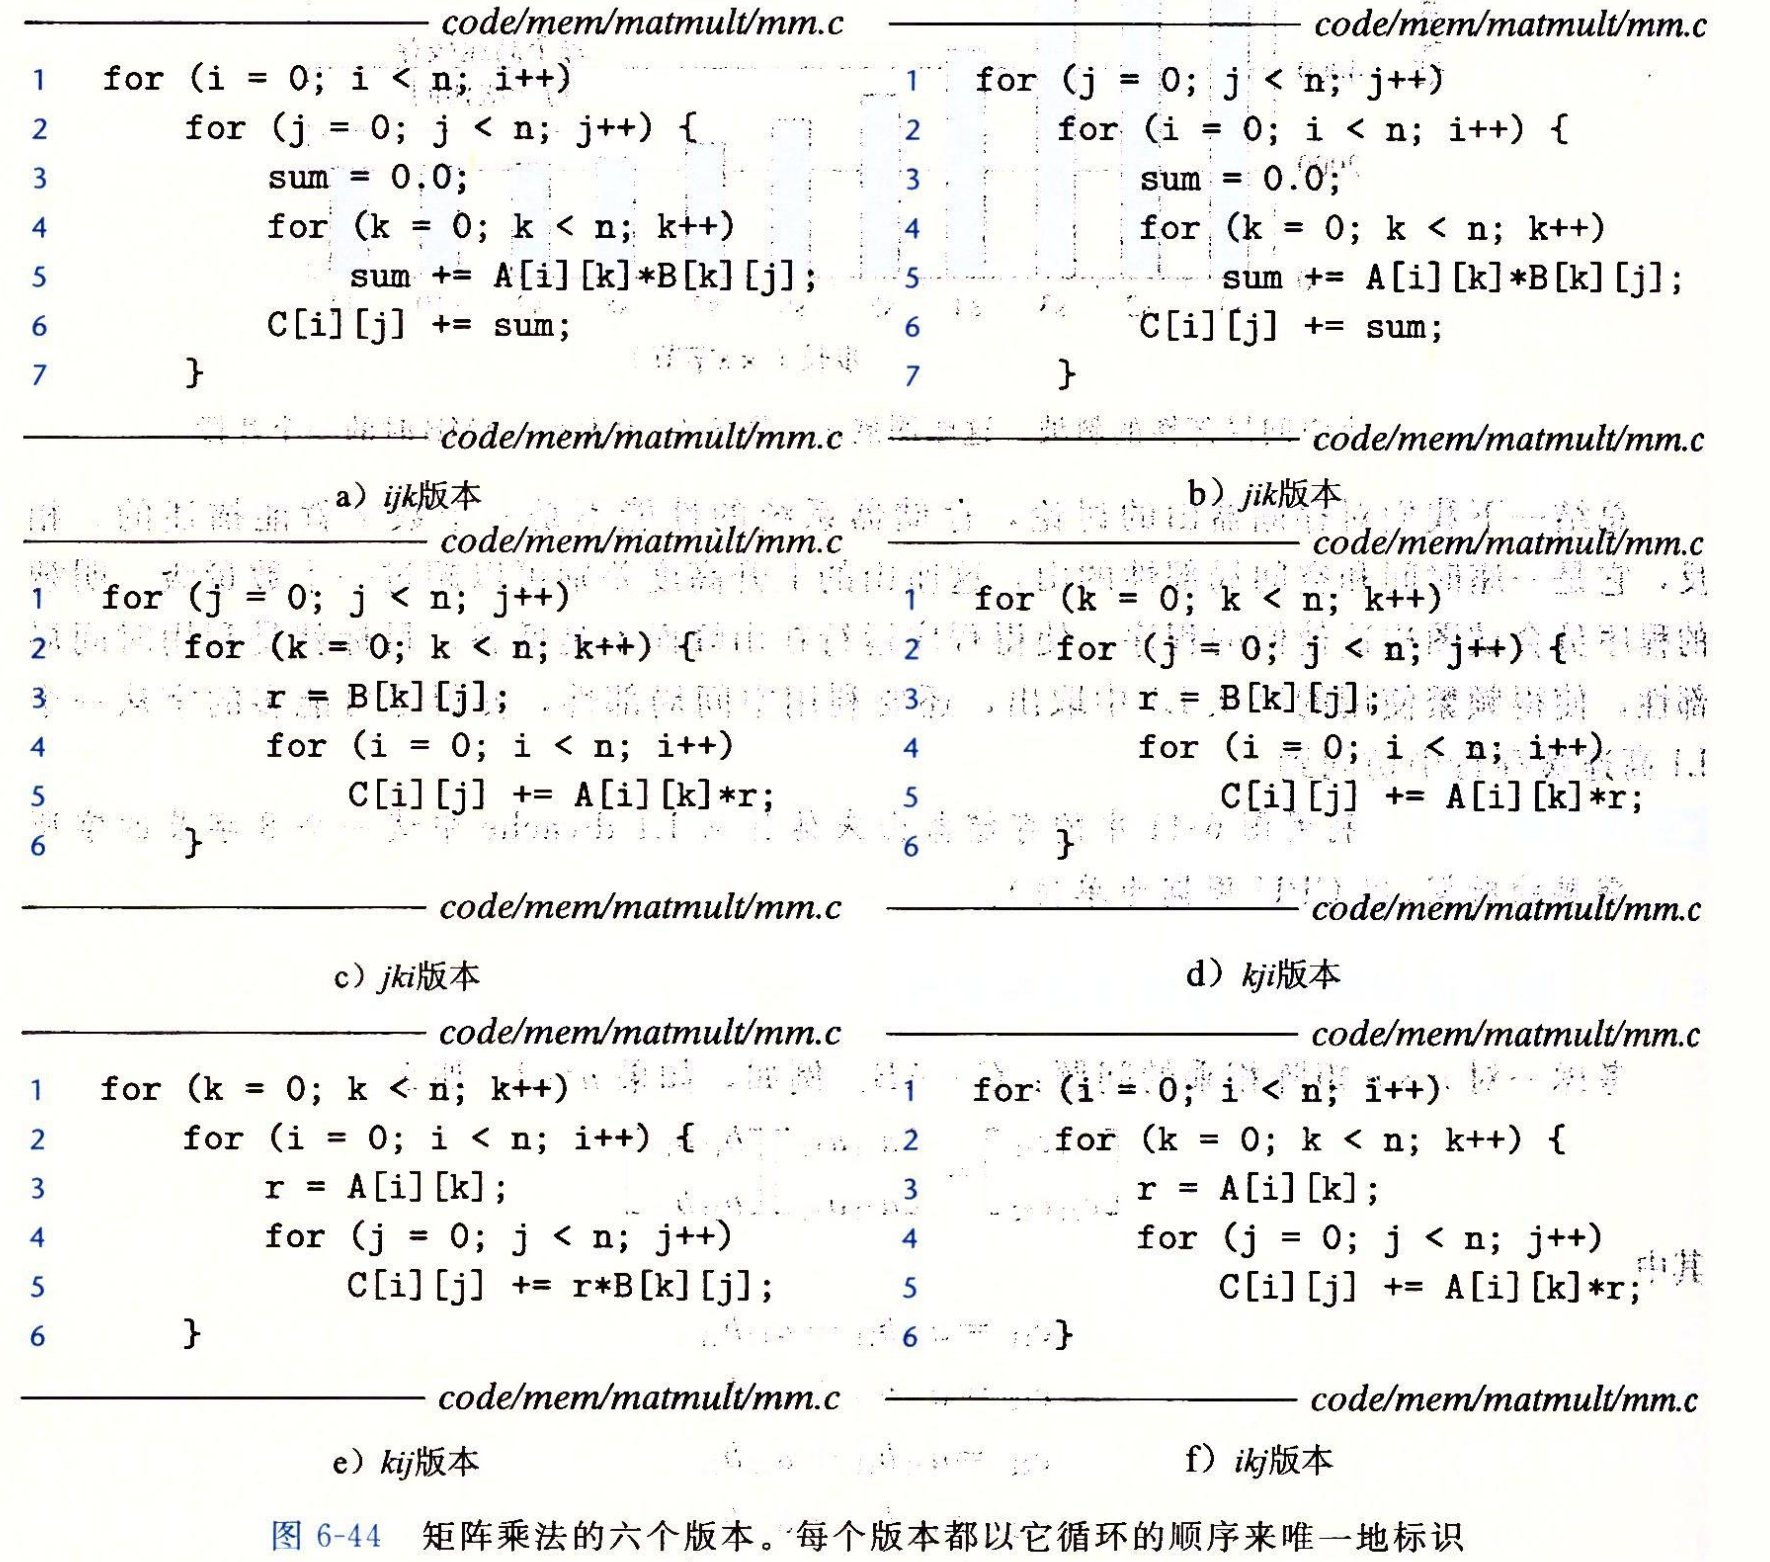
\includegraphics[scale=0.25]{矩阵乘法.png}
    \caption{矩阵乘法代码示意}
    \label{fig:1.1}
\end{figure}
图\ref{fig:1.1}的代码节选自《深入理解计算机系统》,在书中对于矩阵乘法给出了六个版本的算法,但算法中$i,j,k$变量的不同顺序仅仅是对访问内存的次数有影响\footnote[1]{至于为什么交换变量顺序会对访问内存有影响,这里涉及到了程序的局部性原理,已超出了本门课程的范畴,具体请翻阅计算机组成原理相关教材。},对于整体的时间复杂度,依旧为$O(n^3)$,这个算法的时间复杂度在面对两个极为庞大的矩阵进行乘法运算是要消耗非常大的时间的,如果在这种情况下计算矩阵范数是一件十分耗时的事情。

但幸运的是,在许多工程中,我们其实没有必要知道两个矩阵相乘的范数的精确数值(在很多情况下都是这样,我们只需要一个近似的数值,或者说了解到一个上界或者下界就可以,比如上文中提到的时间复杂度大$O$记法,它仅仅描述了一个算法所耗费时间的最坏情况,即一个上界),在这种情况下,矩阵的相容性就会起到作用,计算两个单独的矩阵的范数再相乘一定比计算两个矩阵先相乘再求范数省时。\footnote[2]{关于算法的时间复杂度,如何衡量一个计算机算法的好坏,具体请翻阅计算机算法方面的教材。}
\subsection{常见矩阵范数的相容性}
在了解了何为矩阵范数相容的概念后,接下来就要讨论常见矩阵范数(矩阵1-范数,矩阵2-范数和矩阵无穷范数)的相容性了。
\subsubsection{矩阵1-范数的相容性}
前面已经介绍过矩阵1-范数的结构\[\Vert A\Vert_{m_1}=\sum_{j=1}^{n}\sum_{i=1}^{m}|a_{ij}|\]
下面来证明矩阵1-范数是自相容范数:

\begin{proof}
    若证明矩阵1-范数是自相容范数,只需证
    \[\Vert\bs{AB}\Vert_{m_1}\leq \Vert\bs{A}\Vert_{m_1}\Vert \bs{B}\Vert_{m_1}\]

    设$\bs{A}\in\mathbb{P}^{m\times l},\bs{B}\in\mathbb{P}^{l\times n}$,根据矩阵1-范数的定义,有
    \[
    \begin{aligned}
        \Vert\bs{AB}\Vert_{m_1}&=\sum_{i=1}^{m}\sum_{j=1}^{n}|a_{i1}b_{1j}+a_{i2}b_{2j}+\cdots+a_{il}b_{lj}|\ \ \ (\text{矩阵乘法})\\
        &\leq \sum_{i=1}^{m}\sum_{j=1}^{n}(|a_{i1}||b_{1j}|+|a_{i2}||b_{2j}|+\cdots+|a_{il}||b_{lj}|)\ \ \ (\text{绝对值三角不等式})\\
        &=\sum_{i=1}^{m}\sum_{j=1}^n\sum_{k=1}^{l}|a_{ik}||b_{kj}|\ \ \ (\text{用一个连加号概括上式})
    \end{aligned}
    \]
    
    交换一下连加号的顺序,原式变为
    \[
        \sum_{k=1}^{l}\sum_{i=1}^{m}\sum_{j=1}^{n}|a_{ik}||b_{kj}|
    \]

    由于连加号的计算是由内向外计算的,因此会首先计算$\sum_{j=1}^{n}|a_{ik}||b_{kj}|$,这个时候会发现$a_{ik}$并没有出现下标$j$,也就是说$|a_{jk}|$并不会受$j$的影响,因此,在$\sum_{j=1}^{n}|a_{ik}||b_{kj}|$中,$|a_{ik}|$可以被认为是一个公因子提到公式外面去,则原式可以变为
    \[\sum_{k=1}^{l}\sum_{i=1}^{m}|a_{ik}|\sum_{j=1}^{n}|b_{kj}|\]

    此时观察$\sum_{i=1}^{m}|a_{ik}|\sum_{j=1}^{n}|b_{kj}|$,会发现$\sum_{j=1}^{n}|b_{kj}|$并不受$i$的影响,因此可以把这部分整体当做一个公因式提到外面,于是式子就会变成
    \[\sum_{k=1}^{l}\left[\left(\sum_{i=1}^{m}|a_{ik}|\right)\left(\sum_{j=1}^{n}|b_{kj}|\right)\right]\]

    这里,$\left(\sum_{i=1}^{m}|a_{ik}|\right)$叫做$A$的\textbf{绝对列和},$\left(\sum_{j=1}^{n}|b_{kj}|\right)$叫做$B$的\textbf{绝对行和},这两个概念在下一节算子范数中还会有应用。

    如果想继续提公因式,需要对式子进行放缩,这里引入矩阵$A$的矩阵1-范数,上式变为
    \[\sum_{k=1}^{l}\left(\sum_{j=1}^{n}|b_{kj}|\right)\left(\sum_{k=1}^{l}\sum_{i=1}^{m}|a_{ik}|\right)\]

    这相当于是在原本$A$矩阵的绝对列和的基础上把所有的$A$元素相加,显然结果更大,因此有如下不等关系
    \[\sum_{k=1}^{l}\left[\left(\sum_{i=1}^{m}|a_{ik}|\right)\left(\sum_{j=1}^{n}|b_{kj}|\right)\right]\leq\sum_{k=1}^{l}\left(\sum_{j=1}^{n}|b_{kj}|\right)\left(\sum_{k=1}^{l}\sum_{i=1}^{m}|a_{ik}|\right)\]

    这种情况下可以发现,$\left(\sum_{k=1}^{l}\sum_{i=1}^{m}|a_{ik}|\right)$并不受$\sum_{k=1}^{l}\left(\sum_{j=1}^{n}|b_{kj}|\right)\left(\sum_{k=1}^{l}\sum_{i=1}^{m}|a_{ik}|\right)$中最外层的连加号$\sum_{k=1}^{l}$的影响,因此$\left(\sum_{k=1}^{l}\sum_{i=1}^{m}|a_{ik}|\right)$又是一个公因式,将其提出,最后式子变为
    \[\sum_{k=1}^{l}\left[\left(\sum_{i=1}^{m}|a_{ik}|\right)\left(\sum_{j=1}^{n}|b_{kj}|\right)\right]\leq\left(\sum_{k=1}^{l}\sum_{i=1}^{m}|a_{ik}|\right)\left(\sum_{k=1}^{l}\sum_{j=1}^{n}|b_{kj}|\right)\]

    注意到不等式右侧就是$A$矩阵的矩阵1-范数和$B$矩阵的矩阵1-范数,因此得到了
    \[\Vert\bs{AB}\Vert_{m_1}\leq\Vert\bs{A}\Vert_{m_1}\Vert\bs{B}\Vert_{m_1}\]

    也就说明矩阵1-范数是自相容范数,证毕。
\end{proof}
\subsubsection{矩阵2-范数的相容性}
前面已经介绍过矩阵2-范数的结构
\[\Vert\bs{A}\Vert_{m_2}=\left(\sum_{j=1}^{n}\sum_{i=1}^{m}|a_{ij}|^2\right)^{\frac{1}{2}}\]
下面来证明矩阵2-范数是自相容范数:

\begin{proof}
    若想证矩阵2-范数是自相容范数,只需证\[\Vert\bs{AB}\Vert_{m_2}^2\leq\Vert\bs{A}\Vert_{m_2}^2\cdot\Vert\bs{B}\Vert_{m_2}^2\]

    根据矩阵2-范数的定义,有
    \[\begin{aligned}
        \Vert\bs{AB}\Vert^2_{m_2}&=\sum_{i=1}^{m}\sum_{j=1}^{n}|a_{i1}b_{1j}+a_{i2}b_{2j}+\cdots+a_{il}b_{lj}|^2\\
        &\leq\sum_{i=1}^{m}\sum_{j=1}^{n}\left[|a_{i1}||b_{1j}|+\cdots+|a_{il}||b_{lj}|\right]^2\\
        &=\sum_{i=1}^{m}\sum_{j=1}^{n}\left(\sum_{k=1}^{l}|a_{ik}||b_{kj}|\right)^2
    \end{aligned}
    \]
    
    前面三步的方法跟证明矩阵1-范数是自相容范数的流程是一样的,接下来是不一样的
    
    根据Cauchy不等式,有
    \[
        \begin{aligned}
            \Vert\bs{AB}\Vert_{m_2}^2\leq\sum_{i=1}^{m}\left[\sum_{j=1}^{n}\left(\sum_{k=1}^{l}|a_{ik}|^2\right)\left(\sum_{k=1}^{l}|b_{kj}|^2\right)\right]
        \end{aligned}
    \]

    请注意不等式右侧的$\sum_{j=1}^{n}\left(\sum_{k=1}^{l}|a_{ik}|^2\right)\left(\sum_{k=1}^{l}|b_{kj}|^2\right)$这一部分,依旧是由于计算连加是从内向外计算的,因此项$\sum_{k=1}^{l}|a_{ik}|^2$并不受$\sum_{j=1}^{n}$中$j$的影响,故可以当作公因式提出,如此式子就变为了
    \[\Vert\bs{AB}\Vert_{m_2}^2\leq\sum_{i=1}^{m}\left(\sum_{k=1}^{l}|a_{ik}|^2\right)\left(\sum_{j=1}^{n}\sum_{k=1}^{l}|b_{kj}|^2\right)\]
    
    此时注意到在不等式的右侧,项$\sum_{j=1}^{n}\sum_{k=1}^{l}|b_{kj}|^2$依旧不受$\sum_{i=1}^{m}$中$i$的影响,故整体可以当作公因式提出,如此式子就变成了
    \[\Vert\bs{AB}\Vert_{m_2}^2\leq\left(\sum_{i=1}^{m}\sum_{k=1}^{l}|a_{ik}|^2\right)\left(\sum_{j=1}^{n}\sum_{k=1}^{l}|b_{kj}|^2\right)\]

    即

    \[\Vert\bs{AB}\Vert_{m_2}^2\leq\Vert\bs{A}\Vert_{m_2}^2\Vert\bs{B}\Vert_{m_2}^2\]

    故矩阵2-范数是自相容范数,证毕。
\end{proof}

矩阵2-范数也叫Frobenius范数,其也是用途最多的一种范数,矩阵2-范数还有下面的性质
\begin{them}{矩阵2-范数(Frobenius范数)的性质}{thm:2.2.1}
    设$A\in\mathbb{P}^{n\times n}$,
    \begin{enumerate}
        \item 若$\bs{A}=(a_1, a_2,\cdots,a_n)$,则\[\Vert\bs{A}\Vert^2_F\overset{\textcircled{1}}{=}\Vert\bs{A}\Vert_{m_2}^2\overset{\textcircled{2}}{=}\sum_{i=1}^{n}\Vert a_i\Vert_2^2\]
        其中,$\Vert a_i\Vert_2^2=a_i^H a_i$是$\mathbb{P}^n$中的向量范数
        \item $\Vert\bs{A}\Vert_{m_2}^2\overset{\textcircled{3}}{=}\text{tr}(\bs{A}^H\bs{A})\overset{\textcircled{4}}{=}\sum\limits_{i=1}^{n}\lambda_i(\bs{A}^H\bs{A})$
        \item 对任意的酉矩阵$\bs{U}、\bs{V}\in\mathbb{P}^{n\times n}$,有\[
        \Vert\bs{A}\Vert_{m_2}=\Vert\bs{U}^H\bs{A}\bs{V}\Vert_{m_2}=\Vert\bs{U}\bs{A}\bs{V}^H\Vert_{m_2}
        \]
    \end{enumerate}
\end{them}

这里只给出定理\ref{them:thm:2.2.1}中前两条的证明,第三条的证明在后面的酉不变范数中。


\begin{proof}

    $\textcircled{1}$的证明省略,因为这就是定义——矩阵2-范数也叫Frobenius范数,这无需证明。

    $\textcircled{4}$的证明省略,因为根据矩阵特征值与矩阵的迹的关系,矩阵特征值的和就是矩阵的迹,这也无需证明。

    $\textcircled{2},\textcircled{3},\textcircled{4}$的证明如下:
    设矩阵\[\bs{A}=\begin{bmatrix}
        a_{11}&a_{12}&\cdots&a_{1n}\\
        a_{21}&a_{22}&\cdots&a_{2n}\\
        \vdots&\vdots&&\vdots\\
        a_{n1}&a_{n2}&\cdots&a_{nn}
    \end{bmatrix}\]
    
    则\[\bs{A}^H=\begin{bmatrix}
        \bar{a}_{11}&\bar{a}_{21}&\cdots&\bar{a}_{n1}\\
        \bar{a}_{21}&\bar{a}_{22}&\cdots&\bar{a}_{n2}\\
        \vdots&\vdots&&\vdots\\
        \bar{a}_{1n}&\bar{a}_{2n}&\cdots&\bar{a}_{nn}\\
    \end{bmatrix}\]

    则\[\bs{A}^H\cdot \bs{A}=\begin{bmatrix}
        \sum\limits_{i=1}^n|a_{i1}|^2&*&*&*\\
        *&\sum\limits_{i=1}^n|a_{i2}|^2&*&*&\\
        \vdots&\vdots&&\vdots\\
        *&*&*&\sum\limits_{i=1}^n|a_{in}|^2\\
    \end{bmatrix}\]
    \begin{rmk}
        注意,这里的$*$代表的是计算出来的结果,但这部分的结果对于证明过程没有意义,故不进行计算用$*$代替。
    \end{rmk}

    仔细观察便能发现,对角线上的元素分别为:第一列元素的和的平方、第二列元素的和的平方,一直到第n列元素和的平方,这恰恰等于矩阵的矩阵2-范数,而根据矩阵的迹的计算方法,矩阵的迹等于矩阵对角线元素的和,因此,就有了如下等式\[\text{tr}(A^HA)=\sum_{i=1}^{n}\sum_{j=1}^{n}|a_{ij}|^2=\Vert A\Vert_{m2}\]

    至此,性质1与2证毕。
\end{proof}
\subsubsection{矩阵无穷范数的相容性}

矩阵的无穷范数是不相容的,证明不相容,只需要给出一个反例即可,即只需给出两个矩阵$\bs{A,B}$,使得\[\Vert\bs{AB}\Vert_{m_{\infty}}\nleq\Vert\bs{A}\Vert_{m_\infty}\Vert\bs{B}\Vert_{m_\infty}\]
即可

事实上,若\[
\begin{aligned}
    \bs{A=B}=\begin{bmatrix}
        0&1\\
        1&1
    \end{bmatrix}
\end{aligned}
\]
则\[
\begin{aligned}
    \bs{AB}=\begin{bmatrix}
        0&1\\
        1&1
    \end{bmatrix}^2=\begin{bmatrix}
        1&1\\
        1&2
    \end{bmatrix}
\end{aligned}
\]
故
\[\Vert\bs{AB}\Vert_{m_{\infty}}=2,\ \ \ \Vert\bs{A}\Vert_{m_{\infty}}\Vert\bs{B}\Vert_{m_{\infty}}=1,\ \ \ \Vert\bs{AB}\Vert_{m_{\infty}}>\Vert\bs{A}\Vert_{m_\infty}\Vert\bs{B}\Vert_{m_\infty}\]

因此,矩阵的无穷范数不是自相容范数。
\subsection{酉不变范数}
酉不变范数就是定理\ref{them:thm:2.2.1}中的性质3,下面给出其证明:

\begin{proof}
    \[
    \begin{aligned}
        \Vert\bs{UA}\Vert^2_{m_2}&=\text{tr}\left[(\bs{UA})^H\bs{UA}\right]\\
        &=\text{tr}\left[\bs{A}^H\bs{U}^H\bs{UA}\right](\text{注意到}\bs{U}^H\bs{U}=\bs{E})\\
        &=\text{tr}\left[\bs{A}^H\bs{A}\right]
    \end{aligned}
    \]

    \[
    \begin{aligned}
        \Vert\bs{AV}\Vert^2_{m_2}&=\text{tr}\left[(\bs{AV})^H\bs{AV}\right]\\
        &=\text{tr}\left[\bs{V}^H\bs{A}^H\bs{AV}\right](\text{注意到}\bs{V}^H=\bs{V}^{-1})\\
    \end{aligned}
    \]
    根据矩阵相似的定义,注意到
    \[
        \bs{V^{-1}A^HAV}\sim\bs{A}^H\bs{A}    
    \]
    故\[\begin{aligned}
        \text{原式}=\text{tr}\left[\bs{A}^H\bs{A}\right](\text{因为矩阵相似,故特征值相等,因此矩阵的迹也相等})
    \end{aligned}\]
    证毕。
\end{proof}


在上面的过程中,分别利用酉矩阵与其共轭转置相乘为单位阵以及酉矩阵与其共轭转置互为逆矩阵从而导出矩阵相似的性质进行推导,将上面的两种情况合成在一起就是定理\ref{them:thm:2.2.1}中的第三条的所有。

\section{算子范数}
本章的最后一个大知识点为将要讨论的算子范数,算子范数成功的将向量范数与矩阵范数联系在一起,如此便可通过向量范数来定义矩阵的算子范数。
\subsection{向量范数与矩阵范数的相容关系}

在前面的两个小节中,我们讨论了向量范数和矩阵范数,我们在引入矩阵范数的时候,是通过与向量范数相似的方式来定义矩阵范数,可如果将二者放在一起,他们的相容性关系是如何的呢?

\begin{defn}{矩阵范数与向量范数相容}{def:2.3.1}
    设$\Vert\bs{\cdot}\Vert_{a}$是$\mathbb{P}^n$上的向量范数,$\Vert\bs{*}\Vert_m$是$\mathbb{P}^{n\times n}$上的矩阵范数,且\[\Vert\bs{Ax}\Vert_a\leq \Vert\bs{A}\Vert_m\Vert\bs{x}\Vert_a\]
    则称$\Vert\bs{*}\Vert_m$为与向量范数$\Vert\bs{\cdot}\Vert_a$相容的矩阵范数
\end{defn}

定义\ref{def:def:2.3.1}描述了矩阵范数与向量范数相容的条件,接下来我们来看两个例子:
\begin{example}
    设$\bs{x}\in \mathbb{P}^n, \bs{A}\in\mathbb{P}^{n\times n}$,则\[\Vert\bs{A}\Vert_{m_1}=\sum_{j=1}^{n}\sum_{i=1}^{n}|a_{ij}|\]是与向量范数$\Vert\cdot\Vert_1$相容的矩阵范数。
\end{example}
\begin{solution}
    证明方法与前文证明矩阵1-范数是自相容范数思路相似,只需要将$\bs{B}$矩阵换为向量$\bs{x}$即可,故不赘述。
\end{solution}

\begin{example}
    设$x\in\mathbb{P}^n, A\in \mathbb{P}^{n\times n}$,则$\Vert\bs{A}\Vert_{m_2}$是与$\Vert\bs{x}\Vert_2$相容的矩阵范数
\end{example}
\begin{solution}
    证明方法与前文证明矩阵2-范数是自相容范数思路相似,只需要将$\bs{B}$矩阵换为向量$\bs{x}$即可,故不赘述。
\end{solution}


可是我们知道,向量范数有很多种(参考介绍向量范数的$p-$范数),那对于任意一种向量范数,是否也存在与该向量范数相容的矩阵范数呢?这就是下面要介绍的算子范数:

\subsection{算子范数}
下面给出算子范数的定义:
\begin{defn}{算子范数的定义}{def:2.3.2}
    设$\Vert\bs{x}\Vert_a$是$\mathbb{P}^n$上的向量范数,$\bs{A}\in\mathbb{P}^{n\times n}$,则\[\Vert\bs{A}\Vert_a=\max\limits_{\bs{x}\neq \bs{0}}\frac{\Vert\bs{Ax}\Vert_a}{\Vert\bs{x}\Vert_a}\]
    是与向量范数$\Vert\bs{x}\Vert_a$相容的矩阵范数,并且称该矩阵范数是从属于向量范数$\Vert\bs{x}\Vert$的算子范数。
\end{defn}

定义\ref{def:def:2.3.2}说了两件事情:算子范数是与定义它的向量范数是相容的;同时,说了这个公式代表的事算子范数,为什么算子范数是与定义它的向量范数是相容的呢?证明如下:

\begin{proof}
    由算子范数的定义,有\[\Vert\bs{A}\Vert_a=\max\limits_{\bs{x}\neq \bs{0}}\frac{\Vert\bs{Ax}\Vert_a}{\Vert\bs{x}\Vert_a}\]
    
    那就会有如下关系:
    \[\Vert\bs{A}\Vert_a=\max\limits_{\bs{x}\neq \bs{0}}\frac{\Vert\bs{Ax}\Vert_a}{\Vert\bs{x}\Vert_a}\geq\frac{\Vert\bs{Ax}\Vert_a}{\Vert\bs{x}\Vert_a}\]

    化简一下,就会有\[\Vert\bs{Ax}\Vert_a\leq \Vert\bs{A}\Vert_a\cdot\Vert\bs{x}\Vert_a\]

    也就成功说明了,算子范数是与定义它的向量范数是相容的,证毕。

\end{proof}
请注意,定义\ref{def:def:2.3.2}还有另外一种形式,即\[\Vert\bs{A}\Vert_a=\max\limits_{\Vert\bs{u}\Vert_a=1}\Vert\bs{Au}\Vert_a\]

两种形式的定义是怎么来的呢?推导如下:
\[\Vert\bs{Ax}\Vert_a=\Vert\bs{A}\cdot\frac{\bs{x}}{\Vert\bs{x}\Vert}\Vert_a\]

令$u=\frac{\bs{x}}{\Vert\bs{x}\Vert_a}$,所以,原式变为\[\max\limits_{\Vert\bs{u}\Vert_a=1}\Vert\bs{Au}\Vert_a\]

接下来,我们给出算子范数是范数的证明:

1. 正定性证明

若$\bs{A}$不为$\bs{0}$,则存在$\bs{x_0}\neq \bs{0}$,使得$\bs{Ax_0}\neq \bs{0}$

因此,$\Vert\bs{Ax_0}\Vert_a>0$,正定性证毕。

2. 齐次性证明

\[\begin{aligned}
\Vert\lambda\bs{A}\Vert_a&=\max\limits_{\bs{x}\neq \bs{0}}\frac{\Vert\lambda|\bs{Ax}|\Vert_a}{\Vert\bs{x}\Vert_a}\\\\
&=\max\limits_{\bs{x}\neq \bs{0}}\frac{|\lambda|\Vert\bs{Ax}\Vert_a}{\Vert\bs{x}\Vert_a}\\
&=|\lambda|\max\limits_{\bs{x}\neq \bs{0}}\frac{\Vert\bs{Ax}\Vert_a}{\Vert\bs{x}\Vert_a}\\
&=|\lambda|\Vert\bs{A}\Vert_a
\end{aligned}
\]

齐次性证毕。

3. 三角不等式证明
\[
\begin{aligned}
    \Vert\bs{A+B}\Vert_a&=\max\limits_{\bs{x}\neq\bs{0}}\frac{\Vert(\bs{A+B})\bs{x}\Vert}{\Vert\bs{x}\Vert_a}=\max\limits_{\bs{x}\neq\bs{0}}\frac{\Vert\bs{Ax+Bx}\Vert_a}{\Vert\bs{x}\Vert_a}\\
    &\leq \max\limits_{\bs{x}\neq \bs{0}}\frac{\Vert\bs{Ax}\Vert_a+\Vert\bs{Bx}\Vert_a}{\Vert\bs{x}\Vert_a}
\end{aligned}
\]

令$f(\bs{x})=\max\limits_{\bs{x}\neq \bs{0}}\frac{\Vert\bs{Ax}\Vert_a}{\Vert\bs{x}\Vert_a}, g(\bs{x})=\max\limits_{\bs{x}\neq \bs{0}}\frac{\Vert\bs{Bx}\Vert_a}{\Vert\bs{x}\Vert_a}$, 故
\[\begin{aligned}
    \max\limits_{\bs{x}\neq \bs{0}}\frac{\Vert\bs{Ax}\Vert_a+\Vert\bs{Bx}\Vert_a}{\Vert\bs{x}\Vert_a}\leq f(\bs{x})+g(\bs{x})=\Vert\bs{A}\Vert_a + \Vert\bs{B}\Vert_b
\end{aligned}
\]

至此,三角不等式证毕。

\subsubsection{算子范数的相关定理}

\begin{them}{算子范数一定是自相容范数}{them:2.3.1}
    设$\Vert\bs{x}\Vert_a$是$\mathbb{P}^{n}$上的向量范数,$\bs{A,B}\in\mathbb{P}^{n\times n},\Vert\bs{A}\Vert_a$是从属于$\Vert\bs{x}\Vert_a$的算子范数,则它是相容的矩阵范数,即\[\Vert\bs{AB}\Vert_a\leq\Vert\bs{A}\Vert_a\cdot\Vert\bs{B}\Vert_a\]
\end{them}

定理\ref{them:them:2.3.1}表明,任何一个算子范数都是自相容范数,证明如下:

\begin{proof}
    由算子范数定义,有:
    \[\begin{aligned}
    \Vert\bs{AB}\Vert_a&=\max\limits_{\bs{x}\neq \bs{0}}\frac{\Vert\bs{ABx}\Vert_a}{\Vert\bs{x}\Vert_a}\\
    &\leq \max\limits_{\bs{x}\neq \bs{0}}\frac{\Vert\bs{A}\Vert_a\cdot\Vert\bs{Bx}\Vert_a}{\Vert\bs{x}\Vert_a}\\
    &=\Vert\bs{A}\Vert_a\cdot\max\limits_{\bs{x}\neq \bs{0}}\frac{\Vert\bs{Bx}\Vert_a}{\Vert\bs{x}\Vert_a}=\Vert\bs{A}\Vert_a\cdot\Vert\bs{B}\Vert_a
\end{aligned}
\]

证毕。
\end{proof}

上面的定理与讨论当给定向量范数和矩阵时,就能确定与给定向量范数相容的矩阵范数,那如果给定矩阵范数时,能否找到与其相容的向量范数呢?

\begin{them}{}{them:2.3.2}
    设$\Vert\cdot\Vert_m$是相容的矩阵范数,则存在向量范数$\Vert\bs{x}\Vert$,使得\[\Vert\bs{Ax}\Vert\leq\Vert\bs{A}\Vert_m\cdot\Vert\bs{x}\Vert\]
\end{them}

定理\ref{them:them:2.3.2}的证明如下:

\begin{proof}
定义下列向量范数:\[\Vert\bs{x}\Vert=\Vert\bs{xa}^H\Vert_m,\ \ \ (\bs{a\neq\bs{0}})\]

正定性:
由于$\bs{x}\neq \bs{0}$,故$\bs{xa}^H\neq\bs{0}$,因此$\Vert\bs{x}\Vert=\Vert\bs{xa}^H\Vert_m>0$,正定性证毕。


齐次性:
\[\Vert\lambda\bs{x}\Vert=\Vert\lambda\bs{xa}^H\Vert_m\]

右侧的$\Vert\lambda\bs{xa}^H\Vert_m$是一个矩阵范数,由矩阵范数的齐次性,有\[\Vert\lambda\bs{xa}^H\Vert_m=|\lambda|\Vert\bs{xa}^H\Vert_m\]

齐次性证毕。

三角不等式:

\[\begin{aligned}
    \Vert\bs{x_1+x_2}\Vert&=\Vert(\bs{x_1+x_2})\bs{a}^H\Vert_m\\
    &=\Vert\bs{x_1a}^H+\bs{x_2a}^H\Vert_m
\end{aligned}\]

由矩阵范数的三角不等式,有
\[\begin{aligned}
    \Vert\bs{x_1a}^H+\bs{x_2a}^H\Vert_m\leq\Vert\bs{x_1a}^H\Vert_m+\Vert\bs{x_2a}^H\Vert_m=\Vert\bs{x_1}\Vert+\Vert\bs{x_2}\Vert
\end{aligned}\]

三角不等式证毕,因此,我们可以通过给定的矩阵范数找到其相容的向量范数
\end{proof}

\subsubsection{矩阵范数与特征值之间的关系}
\begin{them}{}{them:2.3.3}
    如果$\Vert\cdot\Vert_m: \mathbb{C}^{n\times n}\rightarrow \mathbb{R} $是一相容的矩阵范数,则对任一$\bs{A}\in\mathbb{C}^{n\times n}$,有\[|\lambda_i|\leq \Vert\bs{A}\Vert_m\]其中,$\lambda_i$是$\bs{A}$的特征值。
\end{them}

定理\ref{them:them:2.3.3}指出了矩阵范数和矩阵特征值之间的关系,由此我们可以矩阵特征值来判断矩阵范数,同理也可以根据矩阵范数判断矩阵特征值。

定理\ref{them:them:2.3.3}的证明如下:

\begin{proof}

    根据特征值的定义,对于矩阵$\bs{A}$的任一特征值$\lambda_i$,有\[\bs{Ax}=\lambda_i\bs{x}\]

    因此,有\[\Vert\bs{Ax}\Vert=\Vert\lambda_i\bs{x}\Vert=|\lambda_i|\Vert\bs{x}\Vert\]

    由定理\ref{them:them:2.3.2}, 若矩阵范数相容,则必定存在一个向量的向量范数与之相容,故,有\[\Vert\bs{Ax}\Vert\leq\Vert\bs{A}\Vert_m\Vert\bs{x}\Vert\]

    因此,就有\[|\lambda_i|\Vert\bs{x}\Vert\leq \Vert\bs{A}\Vert_m\Vert\bs{x}\Vert\]

    由于$\Vert\bs{x}\Vert\neq\bs{0}$,因此,两侧可以约掉$\bs{x}$,于是式子就变成了
    \[|\lambda_i|\leq \Vert\bs{A}\Vert_m\]

    证毕。
\end{proof}

\subsection{算子范数的计算}
本小节着重介绍算子范数的计算,由于特殊的定义关系,有时算子范数并不一定能够计算出来,本小节着重介绍算子1-范数,算子2-范数(也叫谱范数)和算子无穷范数的计算。

\subsubsection{算子1-范数的计算}
从属于向量范数$\Vert\bs{x}\Vert_1=\sum_{i=1}^{n}|x_i|$的算子范数为\[\Vert\bs{A}\Vert_1=\max_{j}\sum_{i=1}^{n}|a_{ij}|\]又称为\textbf{极大列和范数}。

这个公式的意思是,首先先分别计算出每一列的绝对列和出来,然后再找出来最大的那个绝对列和,这就是$\max\limits_j$的含义,而不是找到数字最大的那一列。


如何证明这个等式是正确的呢?往常证明等式成立往往是通过从等式的左侧或右侧出发,经过一系列的变形之后推导到了等式的右侧/左侧,证明了等式的成立,但在本节证明等式成立中,我们并不会采用这种方法,而是首先假设等式的左侧小于等于右侧,证明其成立,而后假设等式的左侧大于等于右侧,证明其成立,两者一结合便只有相等这一种选项。

\begin{proof}

    假设$\Vert\bs{A}\Vert_1\leq\max\limits_{j}\sum_{i=1}^{n}|a_{ij}|$,首先证明该不等式的成立。

    根据矩阵与向量的乘法,有\[\Vert\bs{Ax}\Vert_1=\sum_{i=1}^{n}|a_{i1}x_1+a_{i2}x_2+\cdots+a_{in}x_n|\]
    根据绝对值三角不等式,有如下关系\[
    \begin{aligned}
        \sum_{i=1}^{n}|a_{i1}x_1+a_{i2}x_2+\cdots+a_{in}x_n|\leq\sum_{i=1}^{n}\sum_{j=1}^{n}|a_{ij}||x_j|
    \end{aligned}
    \]

    由于多重累加可以交换顺序,因此上面的式子可以变成\[\sum_{j=1}^{n}\sum_{i=1}^{n}|a_{ij}||x_j|\]
    此时,注意到$\sum_{i=1}^{n}|a_{ij}||x_j|$中的$|x_j|$其实并不会受$j$的变化而变化,因此可以当成公因式提出,于是式子就成了\[\sum_{j=1}^{n}(|x_j|\sum_{i=1}^{n}|a_{ij}|)\]

    仔细观察$\sum_{i=1}^{n}|a_{ij}|$,不难发现,这其实就是矩阵$\bs{A}$的绝对列和,接下来,对式子做类似证明矩阵范数相容性那样进行放缩,有
    \[
    \begin{aligned}
        \sum_{j=1}^{n}(|x_j|\sum_{i=1}^{n}|a_{ij}|)&\leq\sum_{j=1}^{n}(|x_j|\cdot\max\limits_{j}\sum_{i=1}^{n}|a_{ij}|)\\
        &=\max\limits_j\sum_{i=1}^{n}|a_{ij}|\cdot\sum_{j=1}^{n}|x_j|
    \end{aligned}
    \]
    注意到$\sum_{j=1}^{n}|x_j|$其实就是向量$\bs{x}$的向量1-范数,因此有\[\max\limits_j\sum_{i=1}^{n}|a_{ij}|\cdot\sum_{j=1}^{n}|x_j|=\max\limits_j\sum_{i=1}^{n}|a_{ij}|\cdot\Vert\bs{x}\Vert_1\]

    整体的式子是这样的:
    \[\Vert\bs{Ax}\Vert_1\leq\max\limits_j\sum_{i=1}^{n}|a_{ij}|\cdot\Vert\bs{x}\Vert_1\]
    移项,于是就有了\[\frac{\Vert\bs{Ax}\Vert_1}{\Vert\bs{x}\Vert_1}\leq\max\limits_j\sum_{i=1}^{n}|a_{ij}|\]
    或许会有人会发现,左侧$\frac{\Vert\bs{Ax}\Vert_1}{\Vert\bs{x}\Vert_1}$缺少了$\max\limits_{\bs{x}\neq\bs{0}}$,这是为什么呢?
    
    因为在证明的过程中,我们假设的是对任意的$\bs{x}\neq\bs{0}$都成立,因此不必加上$\max\limits_{\bs{x}\neq\bs{0}}$

    很好,我们顺利证明出了$\Vert\bs{A}\Vert_1\leq\max\limits_{j}\sum_{i=1}^{n}|a_{ij}|$,接下来继续证明$\Vert\bs{A}\Vert_1\geq\max\limits_{j}\sum_{i=1}^{n}|a_{ij}|$

    由于涉及到某一列的绝对列和最大,所以不妨假设矩阵$\bs{A}$的第$s$列的绝对列和最大,即矩阵$\bs{A}$的形式为\[\bs{A}=[\bs{\alpha_1, \alpha_2, \cdots,\alpha_s,\cdots,\alpha_n}]\]

    此时,取特殊向量$\bs{x_0}=\bs{\varepsilon_s}$,这里的$\bs{\varepsilon_s}$代表的是单位矩阵$\bs{E}$的第$s$列的列向量

    由向量范数以及单位矩阵的性质,不难得出下列等式关系\[\Vert\bs{x_0}\Vert_1=\Vert\bs{\varepsilon_s}\Vert_1=1\]

    左乘一个矩阵$\bs{A}$,有\[\Vert\bs{Ax_0}\Vert_1=\Vert\bs{A\varepsilon_s}\Vert_1=\Vert\bs{\alpha_s}\Vert_1=\max\limits_j\sum_{i=1}^{n}|a_{ij}|\]

    由于$\Vert\bs{x_0}\Vert_1=1$,因此对于上面的等式同时除以$\Vert\bs{x_0}\Vert_1$,对式子结果不影响,但我们得到了\[\frac{\Vert\bs{Ax_0}\Vert_1}{\Vert\bs{x_0}\Vert_1}=\max\limits_j\sum_{i=1}^{n}|a_{ij}|\]

    此时请注意,由算子范数最开始的定义,算子范数其实是需要找出\[\max\limits_{\bs{x}\neq\bs{0}}\frac{\Vert\bs{Ax}\Vert_1}{\Vert\bs{x}\Vert_1}\]
    这个值的范围是限定在整个矩阵中的,而非仅仅某一列或某一行,这是一种全局最大,但是看上面的证明,我们仅仅是找到了矩阵的某一行最大,是一种局部的最大值,全局最大值一定是大于等于局部最大值的,因此,我们有\[\Vert\bs{A}\Vert_1=\max\limits_{\bs{x}\neq\bs{0}}\frac{\Vert\bs{Ax}\Vert_1}{\Vert\bs{x}\Vert_1}\geq\frac{\Vert\bs{Ax_0}\Vert_1}{\Vert\bs{x_0}\Vert_1}=\max\limits_j\sum_{i=1}^{n}|a_{ij}|\]

    由此,我们证明了$\Vert\bs{A}\Vert_1\geq\max\limits_{j}\sum_{i=1}^{n}|a_{ij}|$,结合上面已经证明出的$\Vert\bs{A}\Vert_1\leq\max\limits_{j}\sum_{i=1}^{n}|a_{ij}|$,我们就可以说,$\Vert\bs{A}\Vert_1=\max\limits_{j}\sum_{i=1}^{n}|a_{ij}|$,证明完毕。

\end{proof}

\subsubsection{算子无穷范数的计算}
从属于$\Vert\bs{x}\Vert_{\infty}$的算子范数为\[\Vert\bs{A}\Vert_{\infty}=\max\limits_{i}(\sum_{j=1}^{n}|a_{ij}|)\]
也被称作\textbf{极大行和范数}.

与证明算子1-范数的方式类似,我们依旧需要构建出两个不等式:$\Vert\bs{A}\Vert_{\infty}=\max\limits_{\bs{x}\neq\bs{0}}\frac{\Vert\bs{Ax}\Vert_{\infty}}{\Vert\bs{x}\Vert_{\infty}}\geq\max\limits_{i}(\sum_{j=1}^{n}|a_{ij}|)$和$\Vert\bs{A}\Vert_{\infty}=\max\limits_{\bs{x}\neq\bs{0}}\frac{\Vert\bs{Ax}\Vert_{\infty}}{\Vert\bs{x}\Vert_{\infty}}\leq\max\limits_{i}(\sum_{j=1}^{n}|a_{ij}|)$,并依次证明成立,最后推出不等关系,证明过程如下:

\begin{proof}
    首先证明\[\Vert\bs{A}\Vert_{\infty}=\max\limits_{\bs{x}\neq\bs{0}}\frac{\Vert\bs{Ax}\Vert_{\infty}}{\Vert\bs{x}\Vert_{\infty}}\leq\max\limits_{i}(\sum_{j=1}^{n}|a_{ij}|)\]

    与证明算子1-范数的过程类似,有\[\Vert\bs{Ax}\Vert_{\infty}=\max\limits_{i}|a_{i1}x_1+a_{i2}x_2+\cdots+a_{in}x_n|\]
    根据绝对值三角不等式,有如下关系\[
    \begin{aligned}
        \max\limits_{i}|a_{i1}x_1+a_{i2}x_2+\cdots+a_{in}x_n|\leq\max\limits_{i}\left(\sum_{j=1}^{n}|a_{ij}||x_j|\right)
    \end{aligned}
    \]

    仔细观察$\sum_{j=1}^{n}|a_{ij}|$,不难发现,这其实就是矩阵$\bs{A}$的绝对行和,接下来,对式子做类似证明矩阵范数相容性那样进行放缩,有
    \[
    \begin{aligned}
        \max\limits_{i}\left(\sum_{j=1}^{n}|a_{ij}||x_j|\right)&\leq\max\limits_{i}\left(\sum_{j=1}^{n}|a_{ij}|\cdot\max\limits_j|x_j|\right)\\
        &=\max\limits_i\sum_{j=1}^{n}|a_{ij}|\cdot\max_j|x_j|\\
        &=\left(\max\limits_i\sum_{j=1}^{n}|a_{ij}|\right)\cdot\Vert\bs{x}\Vert_{\infty}
    \end{aligned}
    \]

    整体的式子是这样的:
    \[\Vert\bs{Ax}\Vert_{\infty}\leq\max\limits_{i}\sum_{j=1}^{n}|a_{ij}|\cdot\Vert\bs{x}\Vert_{\infty}\]
    移项,于是就有了\[\frac{\Vert\bs{Ax}\Vert_{\infty}}{\Vert\bs{x}\Vert_{\infty}}\leq\max\limits_i\sum_{j=1}^{n}|a_{ij}|\]
    
    故,只要有$\bs{x}\neq\bs{0}$,就会有上式成立

    接下来,证明\[\max\limits_{\bs{x}\neq\bs{0}}\frac{\Vert\bs{Ax}\Vert_{\infty}}{\Vert\bs{x}\Vert_{\infty}}\geq\max\limits_{i}(\sum_{j=1}^{n}|a_{ij}|)\]

    但与假设最大绝对列和不同的是,我们其实并没有办法通过简单的一个矩阵乘一个行的形式来构造绝对行和,为此,我们采取下面的方式:

    令$\mu=\sum_{j=1}^{n}|a_{sj}|=\max\limits_i\sum_{j=1}^{n}|a_{ij}|$,其中$a_{sj}=|a_{sj}|\cdot e^{i\theta j}\ \ \ (j=1,2,\cdots,n)$ \footnote[1]{这里涉及到了复数的表示形式和欧拉公式的内容,欧拉公式的表示为$e^{i\theta}=\cos\theta+\sin\theta$,根据该公式,复数还可以使用$z=\rho(\cos\theta+i\sin\theta)$的形式表示。}

由于复数表示的性质,可以知道$e^{i\theta j}$的值是永远小于等于1的,构造一个特殊的向量$\bs{z}$,其形式为\[\bs{z}=(e^{-i\theta_1}, e^{-i\theta_2},\cdots,e^{-i\theta_n})\]
由欧拉公式可知,$\Vert e^{i\theta}\Vert=1$,故$\Vert\bs{z}\Vert_{\infty}=1$

故$\Vert\bs{Az}\Vert_{\infty}=\max\limits_{i}|a_{i1}e^{-i\theta_1}+\cdots+a_{in}e^{-i\theta_n}|$

假设矩阵$\bs{A}$的第$s$行的绝对行和最大,即\[\sum_{j=1}^{n}|a_{sj}|=\max_i\sum_{j=1}^{n}|a_{ij}|\]

于是我们有
\[\Vert\bs{Az}\Vert_{\infty}=\max\limits_{i}|a_{i1}e^{-i\theta_1}+\cdots+a_{in}e^{-i\theta_n}|\geq|a_{s1}e^{-i\theta_1}+\cdots+a_{sn}e^{-i\theta_n}|\]

为什么这个不等关系会成立呢,因为$\max\limits_{i}|a_{i1}e^{-i\theta_1}+\cdots+a_{in}e^{-i\theta_n}|$是所有分量的模的最大值,而$|a_{s1}e^{-i\theta_1}+\cdots+a_{sn}e^{-i\theta_n}|$仅仅只是其中一个分量。

注意到\[a_{si}e^{-i\theta_i}=|a_{si}|e^{i\theta_1}\cdot e^{-i\theta_1}=|a_{s1}|\]

所以\[|a_{s1}e^{-i\theta_1}+\cdots+a_{sn}e^{-i\theta_n}|=|a_{s1}|+|a_{s2}|+\cdots+|a_{sn}|=\max_i\sum_{j=1}^{n}|a_{ij}|\]

故\[\max\limits_{\bs{x}\neq\bs{0}}\frac{\Vert\bs{Ax}\Vert_{\infty}}{\Vert\bs{x}\Vert_{\infty}}\geq\frac{\Vert\bs{Az}\Vert}{\Vert\bs{z}\Vert}=\max\limits_{i}\sum_{j=1}^{n}|a_{ij}|\]

证毕。
\end{proof}


\subsubsection{算子2-范数(谱范数)的计算}
从属于$\Vert\bs{x}\Vert_2$的算子范数(又称为谱范数)为\[\Vert\bs{A}\Vert_2=\sqrt{r(\bs{A}^H\bs{A})}\]

这里出现了一个新的东西:$r(\bs{A}^H\bs{A})$,这是什么东西呢,这个东西表示$\bs{A}^H\bs{A}$的\textbf{谱半径},谱半径的计算方法为:
\[r(\bs{A})=\max\limits_i|\lambda_i|\]即,一个矩阵的谱半径的值就是其特征向量绝对值的最大值。

利用算子范数的定义,即算子2-范数的计算公式为\[\Vert\bs{A}\Vert_2=\max\limits_{\Vert\bs{u}\Vert_2=1}\Vert\bs{Au}\Vert_2=\sqrt{r(\bs{A}^H\bs{A})}\]

这里,依旧只需要证明\[\max\limits_{\Vert\bs{u}\Vert_2=1}\Vert\bs{Au}\Vert_2\geq\sqrt{r(\bs{A}^H\bs{A})}\]和\[\max\limits_{\Vert\bs{u}\Vert_2=1}\Vert\bs{Au}\Vert_2\leq\sqrt{r(\bs{A}^H\bs{A})}\]即可

这里要简单介绍一下Hermite矩阵的概念
\begin{defn}{Hermite矩阵}{}
    设$\bs{A}\in\mathbb{C}^{n\times n}$,若$\bs{A}^H=\bs{A}$,则称$\bs{A}$是Hermite矩阵;若$\bs{A}^H=\bs{-A}$,则称$\bs{A}$是反Hermite矩阵。
\end{defn}
Hermite矩阵还拥有如下性质(这里只写后面需要用到的,具体更多的性质请看后面的相关内容):
\begin{itemize}
    \item $\bs{A}$是正定矩阵
    \item $\bs{A}$的特征值全为正实数
\end{itemize}

因此,对于这里的谱范数,我们不妨设矩阵$\bs{A}^H\bs{A}$的特征值有如下关系:\[\lambda_1\geq\lambda_2\geq\cdots\geq\lambda_n\geq0\]

这里$\lambda_1,\lambda_2,\cdots,\lambda_n$分别为单位特征向量$x_1, x_2,\cdots,x_n$对应的特征值,又由于矩阵$\bs{A}^H\bs{A}$是Hermite矩阵,故其所有的特征向量均正交。

故\[r(\bs{A}^H\bs{A})=\lambda_1\]

任取$\bs{u}=a_1x_1+a_2x_2+\cdots+a_nx_n$,并且令$\Vert\bs{u}\Vert_2^2=1$

因此,有\[\Vert\bs{u}\Vert_2^2=1\]

\begin{proof}
    先证\[\max\limits_{\Vert\bs{u}\Vert_2=1}\Vert\bs{Au}\Vert_2\leq\sqrt{r(\bs{A}^H\bs{A})}\]

    由定义,有\[
    \begin{aligned}
    \Vert\bs{Au}\Vert_2^2&=\bs{u}^H\bs{A}^H\bs{Au}\\
    &=\bs{u}^H\bs{A}^H\bs{A}(a_1x_1+a_2x_2+\cdots+a_nx_n)\\
    &=\bs{u}^H(a_1\bs{A}^H\bs{A}x_1+a_2\bs{A}^H\bs{A}x_2+\cdots+a_n\bs{A}^H\bs{A}x_n)\\
    &=\bs{u}^H(a_1\lambda_1x_1+a_2\lambda_2x_2+\cdots+a_n\lambda_nx_n)\\
    &=(\bar{a}_1x_1^H+\cdots+\bar{a}_nx_n^H)\cdot(a_1\lambda_1x_1+a_2\lambda_2x_2+\cdots+a_n\lambda_nx_n)\\
    &=\lambda_1|a_1|^2+\lambda_2|a_2|^2+\cdots+\lambda_n|a_n|^2
    \end{aligned}
    \]
    由于最开始的特征值之间的大小关系,我们有:
    \[\begin{aligned}
    \lambda_1|a_1|^2+\lambda_2|a_2|^2+\cdots+\lambda_n|a_n|^2 &\leq\lambda_1(|a_1|^2|a_2|^2+\cdots+|a_n|^2)\\
    &=\lambda_1\Vert\bs{u}\Vert_2^2=\lambda_1
    \end{aligned}\]

    即\[\Vert\bs{Au}\Vert_2^2\leq \lambda_1=r(\bs{A}^H\bs{A})\]

    接下来证明\[\max\limits_{\Vert\bs{u}\Vert_2=1}\Vert\bs{Au}\Vert_2\geq\sqrt{r(\bs{A}^H\bs{A})}\]

    由特征值和特征向量的定义,有\[\bs{A}^H\bs{A}\bs{x_1}=\lambda_1\bs{x_1}\]

    等式左右两侧同时乘$\bs{x}_1^H$,有\[\bs{x}_1^H\bs{A}^H\bs{A}\bs{x}_1=\lambda_1\bs{x}_1^H\bs{x_1}^H\bs{x_1}=\lambda_1\]

    即\[\max\limits_{\Vert\bs{u}\Vert_2=1}\Vert\bs{Au}\Vert_2^2\geq\Vert\bs{Ax_1}\Vert_2^2=\bs{x_1}^H\bs{A}^H\bs{A}\bs{x_1}=\bs{x_1}^H\lambda_1\bs{x}=\lambda_1\]

    证毕。

    (数学真好玩,证明真有趣,我要天天学数学数学😇)
\end{proof}

\subsubsection{谱范数的其他性质}
首先介绍谱范数的酉不变性质
\begin{them}{酉不变性质}{them:2.3.4}
    设$\bs{A}\in\mathbb{C}^{n\times n}$,则
    \begin{enumerate}
        \item $\Vert\bs{A}\Vert_2=\Vert\bs{A}^H\Vert_2=\Vert\bs{A}^T\Vert_2=\Vert\bar{\bs{A}}\Vert_2$
        \item $\Vert\bs{A}^H\bs{A}\Vert_2=\Vert\bs{A}\bs{A}^H\Vert_2=\Vert\bs{A}\Vert_2^2$
        \item 对任何$n$阶酉矩阵$\bs{U}$和$\bs{V}$,都有\[\Vert\bs{UA}\Vert_2=\Vert\bs{AV}\Vert_2=\Vert\bs{UAV}\Vert_2=\Vert\bs{A}\Vert_2\]
    \end{enumerate}
\end{them}

上面三个性质的证明如下:

\begin{proof}

    性质1:

    $\Vert\bs{A}\Vert_2=\sqrt{r(\bs{A}^H\bs{A})}$
    因此,有$\Vert\bs{A^H}\Vert_2=\sqrt{r[(\bs{A}^H)^H\bs{A}^H]}=\sqrt{r(\bs{A}\bs{A}^H)}=\sqrt{r(\bs{A}^H\bs{A})}=\Vert\bs{A}\Vert_2$

    $\Vert\bs{A^T}\Vert_2=\sqrt{r[(\bs{A}^T)^H\bs{A}^T]}=\sqrt{r(\bs{A}\bs{A}^H)^T}=\sqrt{r(\bs{A}\bs{A}^H)}=\Vert\bs{A}^H\Vert_2$

    由于$\bar{\bs{A}}=\bs{(\bs{A}^T)}^H$,矩阵的转置与求共轭均不会影响矩阵的范数,因此显然相等,性质1证明完毕。

    性质2:

    $\Vert\bs{A}^H\bs{A}\Vert_2=\sqrt{r[(\bs{A}^H\bs{A})^H\bs{A}^H\bs{A}]}=\sqrt{r(\bs{A}^H\bs{A})^2}=r(\bs{A}^H\bs{A})=\Vert\bs{A}\Vert_2^2$

    性质3:

    性质3的证明方式与矩阵范数中的酉不变范数的证明方式类似,在这里不再赘述

\end{proof}

接下来介绍谱范数的下一条性质:
\begin{them}{}{them:2.3.5}
    设$\bs{A}\in\mathbb{C}^{n\times n}$,则
    \begin{itemize}
        \item $\Vert\bs{A}\Vert_2=\max\limits_{\Vert\bs{x}\Vert_2=\Vert\bs{y}\Vert_2=1}|\bs{y}^H\bs{A}\bs{x}|$
        \item $\Vert\bs{A}\Vert_2^2\leq \Vert\bs{A}\Vert_1\Vert\bs{A}\Vert_{\infty}$
    \end{itemize}
\end{them}

定理\ref{them:them:2.3.5}的证明如下:

对于第一条性质,采用的证明思路是这样的:
\begin{enumerate}
    \item 首先证明右侧的值是一个上界
    \item 其次证明这个上界是可以达到的
\end{enumerate}

首先证明第一项,由Cauchy不等式,有\[|\bs{y}^H(\bs{Ax})|=|<\bs{y}, \bs{Ax}>|\leq\Vert\bs{y}\Vert_2\cdot\Vert\bs{Ax}\Vert_2\]

由范数相容性可知\[\Vert\bs{Ax}\Vert_2\leq\Vert\bs{A}\Vert_2\Vert\bs{x}\Vert_2\]

因此,不等式左右两侧同乘$\Vert\bs{y}\Vert_2$,有\[\Vert\bs{y}\Vert_2\cdot\Vert\bs{Ax}\Vert_2\leq\Vert\bs{y}\Vert_2\cdot\Vert\bs{A}\Vert_2\Vert\bs{x}\Vert_2\]

由于$\Vert\bs{x}\Vert_2=\Vert\bs{y}\Vert_2=1$
因此\[|<\bs{y}, \bs{Ax}>|\leq\Vert\bs{A}\Vert_2\]证明了右侧的确是一个上界,接下来证明该上界可以达到

由算子范数的定义\[\Vert\bs{A}\Vert_2=\max\limits_{\Vert\bs{x}\Vert_2=1}\Vert\bs{Ax}\Vert_2\]

因此,$\exists x_0$,有$\Vert\bs{A}\Vert_2=\Vert\bs{Ax_0}\Vert_2$

对$\bs{Ax_0}$进行单位化, 有$\bs{y}_0=\frac{\bs{Ax_0}}{\Vert\bs{Ax_0}\Vert_2}$

因此,\[|\bs{y}_0^H\cdot\bs{Ax_0}|=|\frac{(\bs{Ax_0})^H\bs{Ax_0}}{\Vert\bs{Ax_0}\Vert_2}|\]

分子恰好是$\bs{Ax_0}$的内积,内积同时也是向量2-范数,故\[|\frac{(\bs{Ax_0})^H\bs{Ax_0}}{\Vert\bs{Ax_0}\Vert_2}|=\frac{\Vert\bs{Ax_0}\Vert_2^2}{\Vert\bs{Ax_0}\Vert_2}=\Vert\bs{Ax_0}\Vert_2=\Vert\bs{A}\Vert_2\]

如此,证明可以达到这个上界

因此\[\max\limits_{\Vert\bs{x}\Vert_2=\Vert\bs{y}\Vert_2=1}|\bs{y}^H\bs{Ax}|=\Vert\bs{A}\Vert_2\]

第二条性质的证明:

$\Vert\bs{A}\Vert_2^2=r(\bs{A}^H\bs{A})$

由于$r(\bs{A}^H\bs{A})=\max\limits_i|\lambda_i|$,故根据定理\ref{them:them:2.3.3},有\[r(\bs{A}\bs{A}^H)\leq\Vert\bs{A}^H\Vert_{\infty}\Vert\bs{A}\Vert_{\infty}\]

这里请回忆一下计算算子无穷范数的时候给出的计算方式,不难发现这里与标准算子无穷范数相比,多了一个转置共轭,算子无穷范数又叫行和范数,转置一下就变成了列和范数,这恰好就是算子1-范数的形式,因此,上式可以变为\[\Vert\bs{A}\Vert_{1}\Vert\bs{A}\Vert_{\infty}\]
即\[\Vert\bs{A}\Vert_2^2=r(\bs{A}^H\bs{A})\leq\Vert\bs{A}\Vert_{1}\Vert\bs{A}\Vert_{\infty}\]

证毕。

\section{酉不变范数}
考试不考,上课没讲,略。
\newpage
\section{矩阵的测度}
考试不考,上课没讲,略。
\newpage
\section{范数的应用}
这一章虽然老师讲了,但是考试不考,主要就是希望各位能够培养一个严谨的精神,一个小小的误差可能会导致求出的结果与理想结果差距甚远,学习方法只需要看老师这一节PPT的几个例子即可。
\newpage
\ifx\allfiles\undefined
\end{document}
\fi